\section{Introduction}

Road traffic injury kills approximately 1.19 million people a year by the World Health Organization's count [1]. Many of those deaths are foreseeable in the seconds before they occur, which is what makes anticipation --- as distinct from detection after the fact --- worth pursuing, as the review of Zhang Y. et al. [2] sets out. The instrument is already in the vehicle: a dashcam holds the primary visual record of the road, the material Moura et al. [3] assembled into a public corpus. It is used almost entirely in retrospect. Whether it can be used prospectively is the question that motivated this work.

We built a training-free system to find out: a zero-shot ensemble scoring each frame of a dashcam clip for collision risk from vision--language similarity, a motion signal and a text-anchored prior, with no accident supervision at any stage. We entered it in a public competition, where the organisers scored it against ground truth we never held. It placed ninth of thirteen.

This paper is not about that system. It is about what we found when we tried to understand the score it received.

The competition scores submissions with a composite metric: a weighted sum of average precision (AP), area under the ROC curve (AUC), and two earliness measures --- time-to-accident (TTA) and stable time-to-accident (STTA) --- each read at a risk threshold of 0.5. The composition is intuitive, and it is becoming common. An anticipator should both separate accident clips from normal driving and raise the alarm early, and summing terms that measure each seems a reasonable way to ask for both.

It is not. AP and AUC are bounded on the unit interval; TTA and STTA are counted in frames and bounded only by the clip, which is 150 frames here. Summing a bounded quantity with an unbounded one lets the unbounded one decide the ranking, and here the timing terms are worth 5.70 times what discrimination contributes to a submission that reads nothing. Worse, the two share a trivial global maximiser: a score that exceeds 0.5 at frame 0 and never falls attains, on every clip, the largest value that clip admits for both. No method that reads the video can exceed it; a method can only match it and then compete on AP and AUC, worth 0.35105 to a blind submission.

So we submitted the constant. It scored 2.35291 against a winning score of 2.50165, matching the eighth-placed team at the precision the leaderboard displays.

The contributions of this work are as follows.

\begin{itemize}
\item
  A measured demonstration on a live benchmark. A video-blind constant matches the eighth-placed private score and exceeds five of thirteen teams, our own included. Every leaderboard score here was computed by the competition's scoring service against ground truth we do not have; derived quantities are our arithmetic on those scores and are marked as such.
\item
  A black-box decomposition. Video-blind probes, built so that unknown terms cancel under differencing, separate a metric whose weights are undisclosed and whose labels are withheld --- recovering the discrimination floor, both timing terms, the slope in the crossing frame, and the accident-onset distribution.
\item
  Evidence that the published definition does not reproduce the scorer. Three curves crossing at the same frame, with identical values at the crossing, score 0.091 apart; under the stated formula they must be equal. The score cannot be computed from the published definition even given the labels.
\item
  A case study in which we are the subject, and a six-point protocol. Our own entry scores below the constant and we report it. The protocol's first item --- report a video-blind control with every result --- costs an afternoon and would have caught this.
\end{itemize}

One point of scope, because this paper prints a number beside other teams'{} numbers. We make no claim about any other submission or published method: we did not re-run anyone's system, and could not have evaluated it if we had, because the labels are withheld from every entrant. Where a leaderboard score is numerically identical to a control's, we state that arithmetic fact and draw one inference --- the metric assigns the two submissions the same value. A whole family of curves receives it, which is precisely the property under examination.

Section 2 reviews the field's evaluation practice, Section 3 states the benchmark and its metric, and Section 4 describes the system, the controls and the probes. Section 5 reports the measurements, Section 6 analyses why the composition fails, and Sections 7 to 9 give the protocol, the limitations and the conclusion.

\begin{enumerate}
\def\labelenumi{\arabic{enumi}.}
\item
  \textbf{RELATED WORK AND EVALUATION PRACTICE}
\end{enumerate}

\emph{\textbf{2.1. Accident anticipation and the origin of its metrics}}

Anticipation is a different and harder problem than detection. In detection the task is to identify what is present in the scene --- a vehicle, a pedestrian, a traffic light --- or what is being done in it, and to classify it; the evidence is in the frame, as in the unsupervised detection work of Liu et al. [17]. In anticipation the object of the prediction is an event that may or may not occur, so the model is asked to reason forward from evidence that is ambiguous and intermittent.

What makes that reasoning possible is the precursor state: a visual signal that danger is developing before anything has happened. A driver on a highway notices that the car fifty metres ahead has drifted twenty centimetres to the right and lost a little speed. No brake has been applied and no collision has occurred, but the drift and the deceleration together indicate drowsiness or distraction. An anticipation model must read signals of the same kind, and the precursors available to it are of the same kind: deviation from an expected vehicle track, congestion patterns, and the projected intersection of two objects extrapolated from their current motion --- the basis on which Yao et al. [18] treat an accident as a departure from predicted trajectories.

Vision-based accident anticipation was posed in its modern form by Chan et al. [4], who introduced the Dashcam Accident Dataset (DAD) together with the measure the field still reports: the interval between the first frame at which a model's risk score crosses a threshold and the annotated onset of the collision. Bao et al. [5] contributed the Car Crash Dataset (CCD) and an uncertainty-based formulation, and Karim et al. [6] gave the reporting convention that most subsequent work adopts --- average precision, mean time-to-accident over thresholds, and time-to-accident at 80\% recall.

It is worth stating plainly what that convention gets right, because this paper is about what happens when it is set aside. It reports a discrimination metric alongside every timing metric, and it reads timing at a fixed operating point of the discrimination metric. A method therefore cannot buy time-to-accident by alarming indiscriminately: the recall constraint holds it to a fixed false-alarm behaviour before its timing is counted at all.

Supervised architectures built on this foundation combine convolutional feature extractors with recurrent or attention-based temporal models trained on labelled dashcam footage, in the line running from Chan et al. [4] and Bao et al. [5] through Karim et al. [6] to Kandacharam et al. [16]. Their shared limitation is dependence on the labelled corpus. Performance degrades on road geometry, weather and traffic culture not represented in training, and collision labels are expensive and rare, which Zhang Y. et al. [2] identify as a persistent constraint on the field.

Self-supervised and unsupervised alternatives reduce that dependence. Yao et al. [18] treat accidents as anomalies in predicted object trajectories, removing the need for accident labels entirely. Liu et al. [17], in SCTNet, apply a causality-guided spatiotemporal diffusion network to unsupervised detection, and Zhong et al. [19] use contrastive feature-consistency representation with soft-label regression for early anticipation on DAD and CCD.

Two lines of work deserve particular attention here, because they anticipate part of this paper's subject. Pjetri et al. [20] train with a self-supervised objective requiring the predicted danger score to be non-decreasing as the collision approaches, and Zou et al. [21] introduce an adaptive monotonic constraint loss with the same intent, evaluated on MM-AU and Nexar. Both are well-motivated responses to score oscillation and we make no criticism of either. But both also illustrate the hazard this paper examines. A risk score constrained not to fall is, by construction, closer to the maximiser of a threshold-crossing timing metric than a score that is free to fall. The metric therefore cannot separate the benefit of the constraint from the artefact of it, and neither paper reports a control that would.

\emph{\textbf{2.2. Vision--language models and training-free anticipation}}

Radford et al. [9] demonstrated with CLIP that contrastive pretraining on 400 million image--text pairs yields a model whose zero-shot classification and retrieval transfer without task-specific supervision. Instruction-tuned multimodal models --- LLaVA, from Liu et al. [11], and the InternVL series of Chen et al. [12] --- extend this to open-ended scene description and reasoning, at substantially higher inference cost per frame. Motion is the other signal these systems draw on: dense optical flow, for which the RAFT estimator of Teed and Deng [10] is the modern standard, yields pixel-level motion fields, while frame differencing is the cheap approximation. Section 4 states which of the two the system examined here uses, and declines to assert an accuracy-for-compute trade-off that was not measured.

Applied to traffic safety, these models have mostly been used for accident understanding rather than anticipation. Zhang R. et al. [15] deploy multimodal large language models for video-based accident analysis, showing that language-level reasoning surfaces causal structure that purely visual models miss. Zhang J. et al. [14] integrate scene-level context with visual perception for risk anticipation. Liao et al. [13] add chain-of-thought reasoning to a multimodal large language model and report improved anticipation. These systems require fine-tuning, a large-model inference pipeline, or both.

Training-free work has appeared very recently. Thakur and Talele [24] combine frame-difference peak detection, Farnebäck optical flow and CLIP prompt matching with no fine-tuning; Saha et al. [22] propose a coarse-to-fine vision--language-model tracking pipeline; and Singh et al. [23] use metadata-aware multi-prompt reasoning. All three target the detection, localisation or classification of an accident in surveillance video, and none reports a time-to-accident metric. Zero-shot anticipation evaluated on a timing metric therefore remains sparse, which is what motivated the system described in Section 4 and why it was submitted to a competition rather than scored locally.

\emph{\textbf{2.3. Corpora}}

The Dashcam Accident Dataset of Chan et al. [4] and the Car Crash Dataset of Bao et al. [5] remain the standard labelled benchmarks and publish their annotations, which is what would make the corrected protocol of Section 7 computable on them. MM-AU, released by Fang et al. [7], is a large ego-view corpus of 11,727 accident videos with object boxes and video--text pairs across 58 accident-reason categories. The Nexar dashcam collision prediction dataset of Moura et al. [3] is a separate resource, by a separate group, of roughly 1,500 clips released for a public challenge. The two are sometimes conflated in the literature and should not be.

The benchmark examined in this paper, released by AUTOPILOT [8], distributes a curated 1,417-clip subset of MM-AU. Its labels are withheld from entrants and exposed only through a leaderboard. That design is legitimate, and it is what makes the measurements of Section 5 third-party rather than self-reported. It also removes every locally computable check an entrant might otherwise apply, a consequence Section 3 develops.

\emph{\textbf{2.4. What the field reports, and what it does not}}

The convention of Karim et al. [6] pairs timing with discrimination and fixes an operating point. Competitions need something that convention does not supply: a total order over submissions. The natural way to obtain one is to sum the metrics into a single score, and that is what the benchmark studied here does, adding two threshold-crossing timing terms to average precision and area under the ROC curve, as the evaluation page of AUTOPILOT [8] sets out.

Summing is where the difficulty enters, and it is a difficulty of type rather than of tuning. Average precision and area under the curve are bounded on the unit interval. A time-to-accident measured in frames is bounded only by the length of the clip. Adding them makes the sum depend on how the corpus was windowed, and lets the unbounded term decide the ranking. Section 6 develops the argument; Section 5 measures its magnitude.

The check that exposes such a problem is a control that does not read the input, and its value has been established repeatedly in adjacent fields. In each case the control was cheap, and in each case nobody had run it. Torralba and Efros [25] showed that image datasets carry signatures strong enough for a classifier to name the dataset a photograph came from, which changed how benchmark results were read. In natural language inference, Gururangan et al. [26] and Poliak et al. [27] showed independently that a model given only the hypothesis --- half of the input --- scores far above chance on SNLI and MNLI, demonstrating that the headline numbers were partly measuring annotation artefacts rather than inference; partial-input baselines became standard practice afterwards. In recommender systems, Ferrari Dacrema et al. [28] found that properly tuned simple baselines matched or beat most recently published neural methods, and evaluation practice in that field changed in consequence.

Accident anticipation has every precondition those episodes had. It reports a timing metric whose maximiser is trivial. It is moving toward composite single-number scores. Its newest benchmarks withhold labels, so an entrant cannot compute the discrimination half at all and must develop against a locally computable proxy --- and the only proxy that is locally computable is the shape of one's own risk curve, which a constant maximises. Yet of the works surveyed in this section that report anticipation results on average precision, area under the curve, time-to-accident or a composite of these, we found none that reports them alongside an input-independent control --- a baseline whose per-frame risk output is a function of the frame index alone. Two of the benchmark papers examined here, those of Moura et al. [3] and Fang et al. [7], publish no anticipation scores of their own and so do not bear on the point. That absence, rather than any defect in any particular method, is what this paper addresses.

This is not to say that the timing metrics have gone unquestioned. Zhao et al. [30] observe that the standard time-to-accident calculation credits a false alarm in a safe scene with the interval to some later, causally unrelated collision, producing what they call artificially inflated estimates. Goldshmidt et al. [31] report that baseline methods on Nexar make physically implausible predictions nine to ten seconds before a collision. Most directly, Caselli et al. [32] publish on Nexar a table in which two established anticipation methods record areas under the curve of 45.5 and 41.0 --- below chance --- beside mean times-to-accident of 10.216 and 10.263 seconds. A method that cannot separate accident clips from normal ones is there credited with ten seconds of anticipation, which is this paper's argument already legible in someone else's results table. What these accounts share is that the pathology is noticed as an anomaly in the numbers of trained models. None of them isolates it, and none reports what a submission that reads nothing would score.

The nearest methodological precedent lies in an adjacent task. Korkut et al. [29] audit four traffic video question-answering benchmarks, MM-AU among them, by running vision--language models blind --- given the question and answer options but no video --- and find that on MM-AU removing the video consistently improves accuracy. That is a control of exactly the kind advocated here, applied to multiple-choice accuracy rather than to per-frame risk. We are not aware of an equivalent control reported for the timing and discrimination metrics used in anticipation, which is the gap this paper fills.

We state the scope of that observation precisely. It covers the works cited in this section whose results tables we were able to inspect directly; four of those we consulted are behind paywalls we could not open, and we exclude them from the count rather than assume. It is not a systematic audit of the field, and we do not present it as one.

\emph{\textbf{2.5. Positioning of this work}}

The contribution of this paper is not an anticipation method. The ensemble described in Section 4 is the instrument that led to the finding and the case study that illustrates it. As a system it is unremarkable, and it placed ninth of thirteen.

What is new is threefold: a measurement, on a live benchmark, of how much of a composite anticipation score a video-blind submission collects; a probe methodology that decomposes such a score from outside a competition, without labels and without knowledge of the weights; and a protocol whose central requirement is that a control be reported.

We are equally explicit about what is not new. Monotonicity constraints on risk scores are prior work, due to Pjetri et al. [20] and Zou et al. [21], and this paper claims none. Training-free pipelines combining CLIP with a motion signal already exist, as Thakur and Talele [24] show. Nor is the general idea that a benchmark can be satisfied by a degenerate submission new, and the specific suspicion that time-to-accident is inflatable has been voiced before by Zhao et al. [30], Goldshmidt et al. [31] and Caselli et al. [32], as has the use of a blind control on an adjacent traffic-video task by Korkut et al. [29]. What is new is the measurement of how far it goes on this class of metric, and the demonstration that the measurement can be made from outside the competition that holds the labels.

\begin{enumerate}
\def\labelenumi{\arabic{enumi}.}
\setcounter{enumi}{1}
\item
  \textbf{THE BENCHMARK AND ITS METRIC}
\end{enumerate}

\emph{\textbf{3.1. The competition}}

The measurements in this paper were made on Zero-shot Accident Anticipation, the public competition hosted on Kaggle by AUTOPILOT [8]. It ran from 17 February to 15 April 2026 and drew 59 entrants, 20 participants and 13 teams across 194 submissions. Late submission remains open and is scored against the same data splits, which is how the experiments of Section 5 were run after the closing date. Every figure in this section was read from the competition's Overview, Evaluation, Data and Leaderboard pages on 31 August 2026.

Two properties make it a suitable instrument for this study. The organisers hold the labels and compute every score, so nothing reported here depends on our own implementation of a metric. And a submission is a plain list of numbers per clip, so it need not contain a model at all --- which is what makes a video-blind control submittable in the first place.

\emph{\textbf{3.2. What the corpus provides}}

The corpus is a curated 1,417-clip subset of the MM-AU corpus of Fang et al. [7]. Every clip is exactly 150 frames at 30 frames per second, five seconds long, and is distributed as a directory of JPEG frames rather than as an encoded video file. Alongside the frames the distribution supplies driver gaze maps and one short text caption per clip. The competition documentation describes five scene categories --- highway, urban, rural, mountainous and tunnel --- together with rare weather (rain, snow, fog) and lighting (night) conditions. There is no training split; the competition is inference-only by design, which is what the word zero-shot denotes in its title.

\emph{\textbf{3.3. What the corpus withholds, and what follows from it}}

The published test file carries five fields: an identifier, a video identifier, a start frame, an end frame, and a caption. There is no label, no accident time and no alert time. Ground truth is held by the organisers and exposed only through the leaderboard.

One consequence deserves emphasis, because the rest of this paper turns on it. Average precision, area under the ROC curve, a false-positive rate, and any time-to-accident measured to a true onset are not computable by any entrant. An entrant who wants to measure progress locally must substitute something, and the only quantities computable from a submission alone are properties of the risk curve's own shape: the frame at which it crosses the threshold, whether it falls back afterwards, how steeply it rises. Section 4 records that we did exactly this --- the encoder in Table 1 was chosen on crossover frame --- and Section 5 measures what that proxy is worth.

A second consequence is worth recording without overstating it. The captions describe outcomes. Seventy-nine distinct captions cover the 1,417 clips, the most frequent being ``lead vehicle stops'' (146 clips), ``a vehicle controls loss'' (144) and ``ego-car controls loss'' (133). They state what happens, and they are supplied at inference time, so a method conditioned on them has access to the outcome it is being asked to anticipate. The system described in this section does not use them; it manufactures its own text anchors from a motion statistic. We identify the hazard and do not quantify it.

\emph{\textbf{3.4. The metric, as published}}

The evaluation page defines the score as a weighted average of four quantities:

score = w\_AP · AP + w\_AUC · AUC + w\_TTA · TTA@0.5 + w\_STTA · STTA@0.5

with the four weights stated to be fixed by the organisers and not disclosed. Positives are accident clips and negatives are normal driving clips; the area under the curve is given in its rank formulation. The two timing terms are defined at a risk threshold of 0.5:

TTA@0.5 = max \{ t\_ai − t\_a \textbar{} p\_t \textgreater{} 0.5, 0 ≤ t\_a ≤ t\_ai \}

STTA@0.5 = max \{ t\_ai − t\_a′ \textbar{} p\_t \textgreater{} 0.5 for all t in [t\_a′, t\_ai] \}

where t\_ai is the accident start frame within the 150-frame clip and t\_a is the first frame at which the risk score exceeds the threshold. STTA additionally requires the score to remain above the threshold continuously from t\_a′ to t\_ai.

Three observations follow from these definitions alone, before any measurement is made.

First, AP and AUC are bounded on the unit interval, while TTA and STTA are counted in frames and bounded only by t\_ai, and hence by how the corpus was windowed. The four terms are not commensurable, and their sum inherits the scale of the larger pair.

Second, both timing terms are maximised by the same trivial submission. A risk score that exceeds 0.5 at frame 0 and never falls has t\_a = 0 and satisfies the continuity condition on every clip, so it attains TTA = STTA = t\_ai, the largest value each clip admits. No submission of any kind can exceed it on either term; a submission can only match it, and then compete on AP and AUC.

Third, neither timing term reads the magnitude of the score, only whether it stands above 0.5. A submission that is barely committed and one that is certain receive identical timing credit, so the metric offers no incentive to calibrate.

\emph{\textbf{3.5. Reproducibility of the submission path}}

Before spending a submission slot, we regenerated the organisers'{} sample submission file from its own parsed values and compared it byte for byte against the distributed file: identical, 1,417 rows of 1,417. This fixes the identifier ordering, the list formatting and the float representation, and it means a scoring anomaly cannot be attributed to our file writer. Every submission reported in Section 5 was additionally checked for length 150, for finiteness, and for range within [0, 1] before upload.

\begin{enumerate}
\def\labelenumi{\arabic{enumi}.}
\setcounter{enumi}{2}
\item
  \textbf{Method: the system under study, the video-blind controls, and the probes}
\end{enumerate}

Pre-crash systems differ from reactive ones in that the prediction must precede the event. This section states the problem, describes the system that was entered, and defines the video-blind controls and the probes with which the metric was later measured.

\begin{enumerate}
\def\labelenumi{\arabic{enumi}.}
\item
  \textbf{Problem Statement:}
\end{enumerate}

The considered problem is anticipating accidents without any training data and it is expected to generalize well only with pretrained knowledge. The formal definition of the problem is as follows:

Let the 5 second dashcam video sequence be defined as a temporally ordered set of frames \(V_{s =}\{ f_{1},f_{2}\ldots\ldots\ldots f_{m}\)\} and the dimension of each frame denotes the RGB observation at time t as \(f_{t} \in \mathbb{R}^{H \times w \times 3}\). The accident anticipation problem thus denotes a learning predictive mapping that predicts the risk score for each frame. The learning predictive mapping is formally denoted as mentioned in equation (1)

\[g\ :\ \mathcal{W}_{t} \longrightarrow \rho_{t} \in \lbrack 0,1\rbrack\ldots\ldots\ldots.(1)\]

\(\rho_{t}\)Where ρ(t) is the predicted probability of an accident, computed without observing one. The risk score should begin near 0 and rise toward 1 before the collision, and the earlier it crosses 0.5 the better the official score. That last clause is not a design preference but a literal description of the metric, and it is this paper's subject: Section 5 shows that a score crossing at frame 0 and never falling collects almost all of what the metric awards.

This problem statement is specifically difficult to solve for the following reasons:

1.~~~~ ~As there are no training data, it becomes impossible to fine-tune the model.

2.~~~~ The clips are diverse in accident type and in condition --- lane changes, rear-end collisions, red-light violations, pedestrians; rain, fog, night, tunnels, mountain roads --- and no training data is available to adapt to any of them.

3.~~~~ The considered dataset is diverse in terms of accident categories, and without any training instances, it might generalize well.

4.~~~~ The four official metrics --- AP, AUC, TTA@0.5 and STTA@0.5 --- must be optimised together, and none of them can be computed by an entrant, because the corpus publishes no labels (Section 3.3).

~

\begin{enumerate}
\def\labelenumi{\arabic{enumi}.}
\setcounter{enumi}{1}
\item
  \textbf{Overall System Architecture:}
\end{enumerate}

PreCrash is modular and decoupled. Three pretrained engines --- a vision--language semantic engine, a motion engine and a text-anchored prior --- run independently, sharing no weights or activations, and are combined only at a late fusion layer. Each is matched to its own representational domain, so no single model carries the whole burden of reasoning about appearance, motion and semantics at once, and any engine can be replaced without disturbing the others. That separation is also what makes the per-modality failure analysis of Section 5.6.1 possible.

\begin{enumerate}
\def\labelenumi{\arabic{enumi}.}
\item
  \emph{System Architecture overview:}
\end{enumerate}

The system takes a 150-frame clip, dispatches it to the three engines in parallel with no inter-stream communication, and combines their per-frame curves in a six-stage pipeline: frame loading, semantic scoring, motion scoring, caption prior, ensemble, and post-processing (Figure 1).

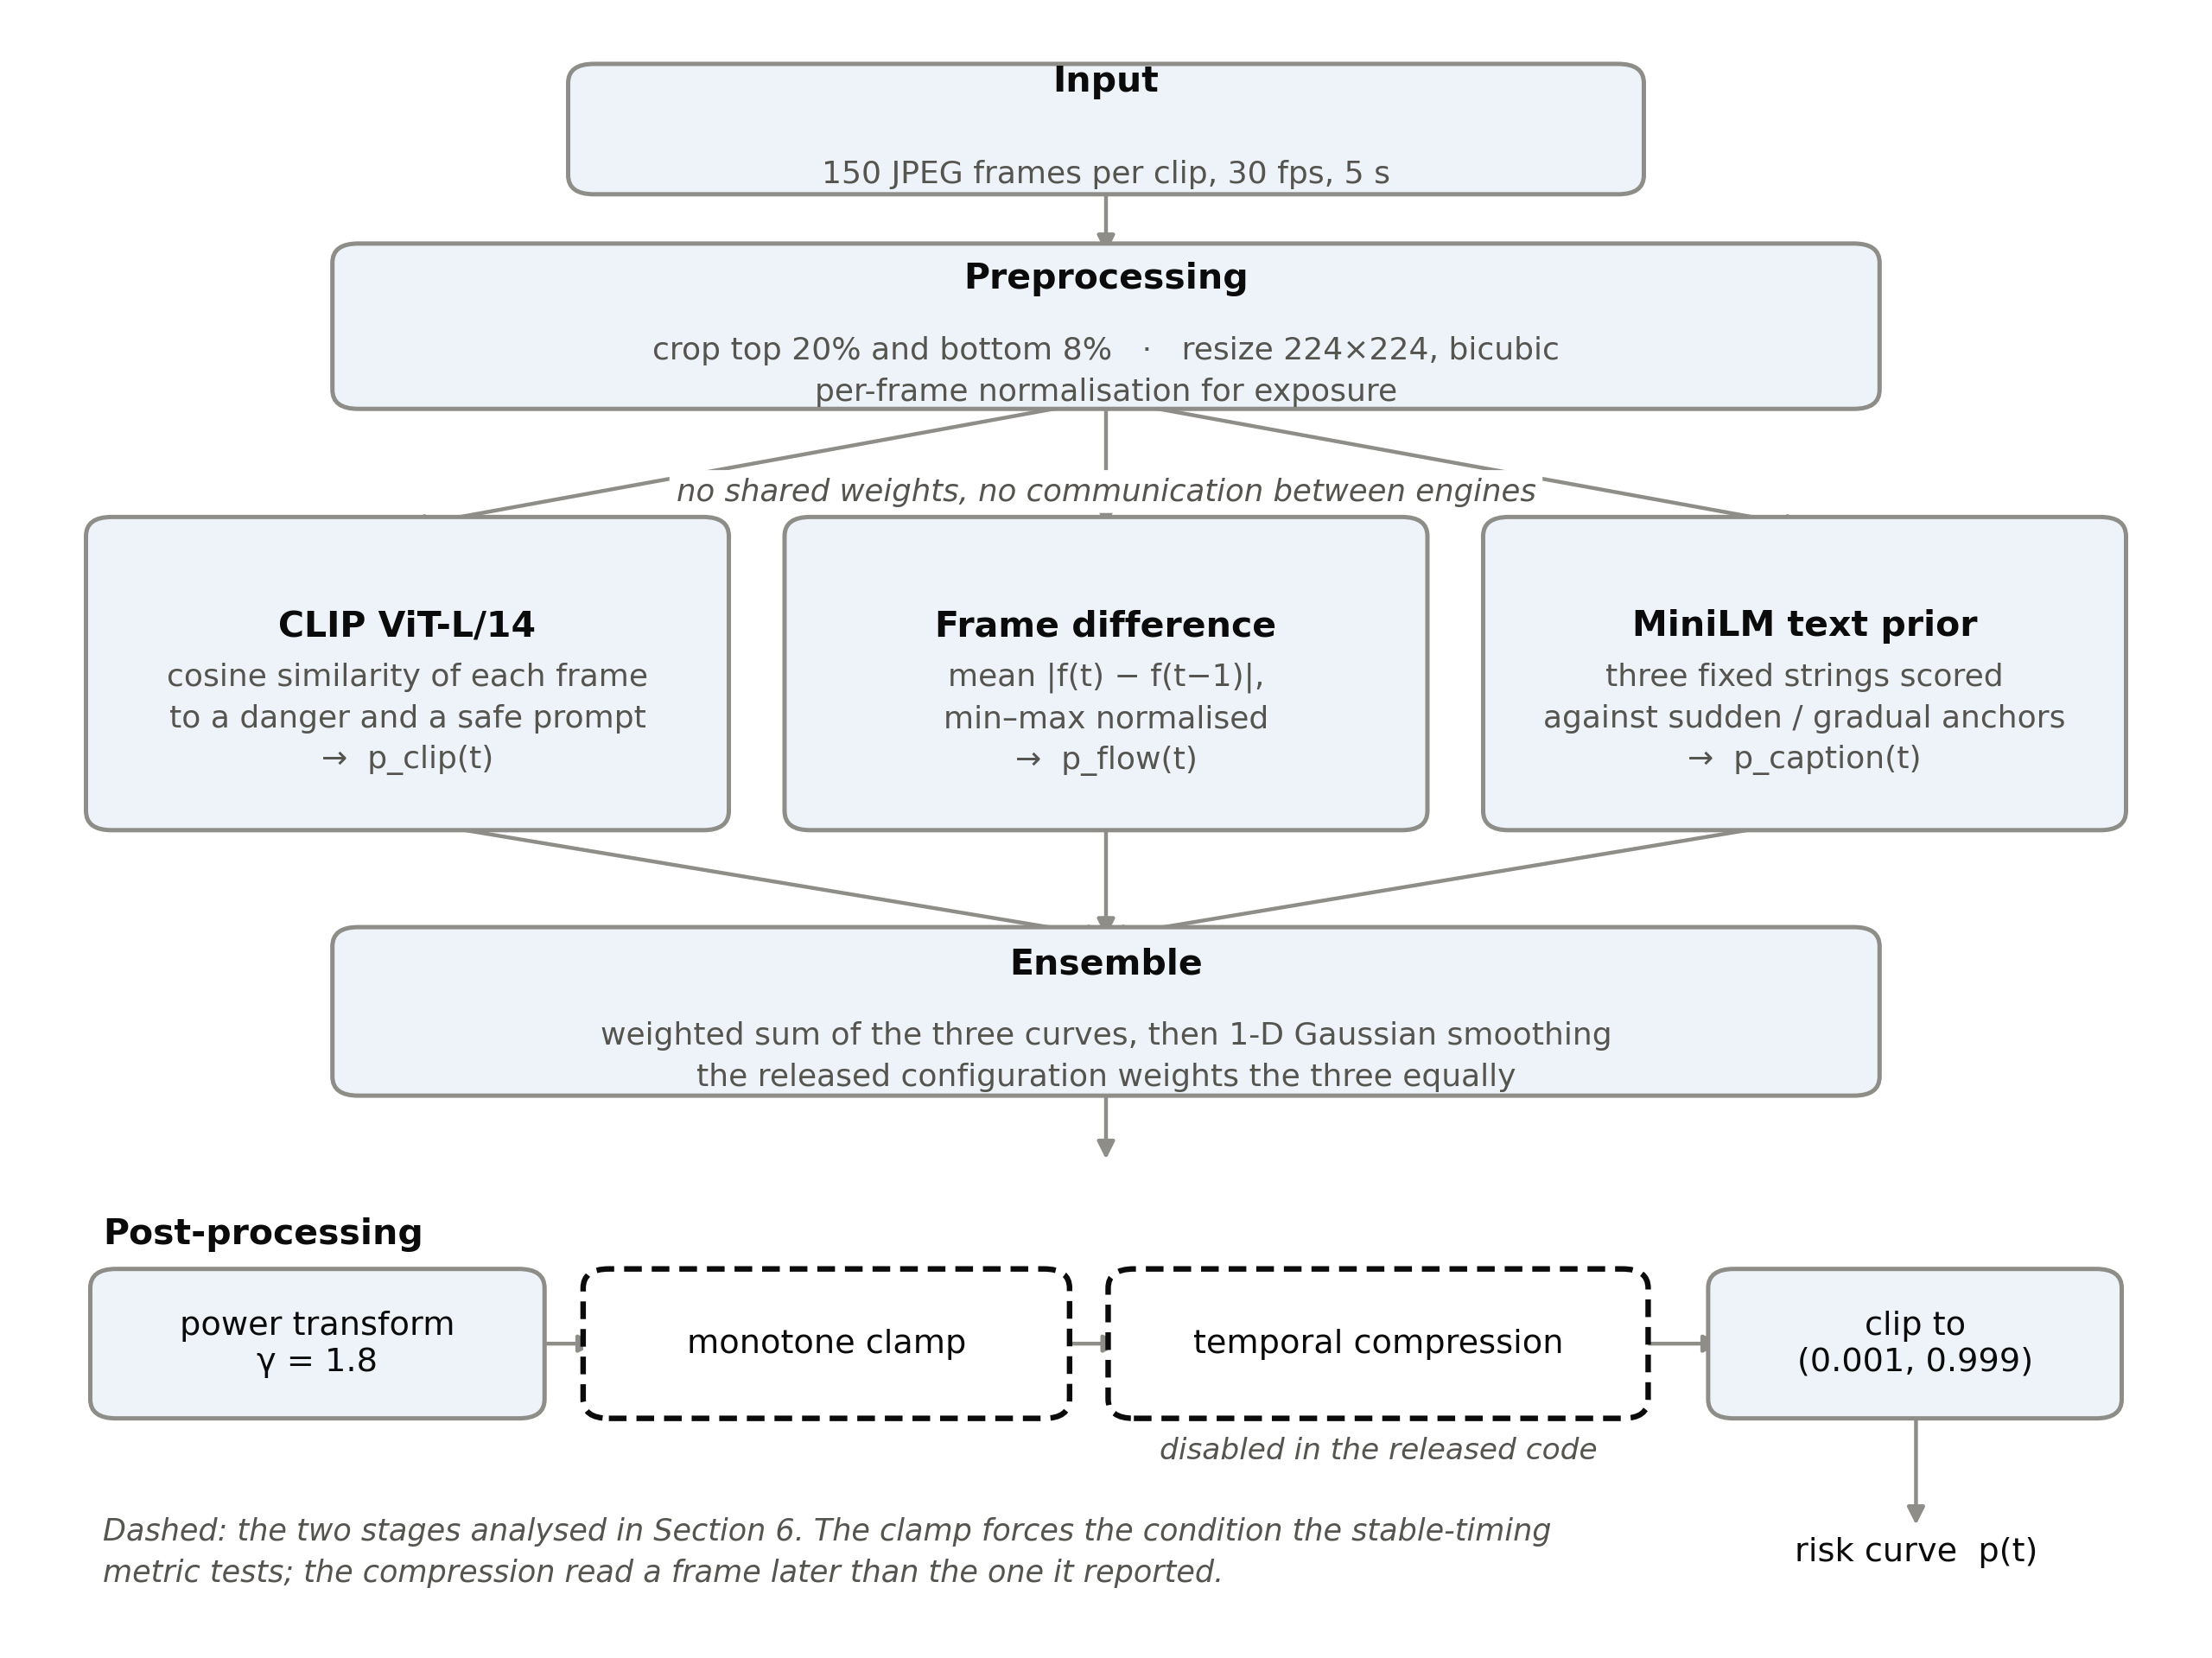
\includegraphics[width=6.26806in,height=4.69869in]{media/image1.png}

\textbf{Figure 1: The pipeline as implemented. Dashed stages are the two analysed in Section 6: the monotone clamp forces the condition the stable-timing metric tests, and the temporal compression reported at each frame a score computed from a later one.}

\begin{enumerate}
\def\labelenumi{\arabic{enumi}.}
\setcounter{enumi}{1}
\item
  \emph{Input and Preprocessing:}
\end{enumerate}

Each clip arrives as 150 JPEG frames at 30 frames per second, five seconds long, with no audio; the distribution also supplies driver gaze maps and one caption per clip. Frames are resized to 224×224 with bicubic interpolation, the upper 20\% and lower 8\% are stripped to remove sky and bonnet, and per-frame normalisation handles exposure variation --- which matters because a zero-shot pipeline cannot adapt to a distribution shift. Homography-based stabilisation against camera shake was specified in the design but is absent from the released code, so the motion signal is computed on unstabilised frames and the shake remains in it. That matters for the frame-difference proxy described below.

\begin{enumerate}
\def\labelenumi{\arabic{enumi}.}
\setcounter{enumi}{2}
\item
  \emph{Parallel Processing:}
\end{enumerate}

The three engines were chosen by trial rather than by training, since no training data exists. The reason for each is given below.

\begin{enumerate}
\def\labelenumi{\arabic{enumi}.}
\item
  CLIP ViT-L/14:
\end{enumerate}

Visual scoring asks whether a frame resembles danger --- which requires reading the scene semantically rather than as pixels. CLIP does this at zero shot because it was pretrained on 400 million image--text pairs and can therefore compare a frame against a danger prompt with no task-specific training. ViT-L/14 was chosen over the smaller variants for its finer spatial detail. Convolutional backbones were rejected because they cannot score a frame against a text prompt without accident-specific training, object detectors because they locate objects rather than assess risk, and the larger instruction-tuned models because their per-frame decoding cost exceeded the compute available.

\begin{enumerate}
\def\labelenumi{\arabic{enumi}.}
\setcounter{enumi}{1}
\item
  \emph{Optical Flow:}
\end{enumerate}

Motion asks a different question: are objects moving as normal physics would predict, or not? Accidents are generally preceded by kinematic abnormality --- a pedestrian stepping out, a sharp deceleration, an unexpected object. The RAFT estimator of Teed and Deng [10] is the more accurate way to capture this, but it did not fit the compute budget available, so a frame-difference proxy was used instead. The trade-off was never measured: an earlier version of this work asserted that frame differencing retains about 90\% of RAFT's sensitivity at about 1\% of its cost, and that figure was an estimate with no ablation behind it. It is withdrawn. Frame difference is computed as follows.

\[flow(t) = mean\left( \left| frame(t) - frame(t - 1) \right| \right)\ldots\ldots\ldots..(1)\]

\subsubsection{\emph{Caption NLP Prior:}}

Vision and motion between them still do not answer what is happening. A text prior adds that: captions translate the scene into language, which can be compared against high-risk action patterns, and sentence encoders trained on large image--text corpora carry enough of that structure to reason about danger without task-specific training. Table 1 records how the encoder was chosen.

\textbf{Table 1: Sentence encoders compared by average crossover frame --- the locally computable proxy, not accuracy. Read with the caveat below.}

\begin{longtable}[]{@{}
  >{\raggedright\arraybackslash}p{(\columnwidth - 4\tabcolsep) * \real{0.3205}}
  >{\raggedright\arraybackslash}p{(\columnwidth - 4\tabcolsep) * \real{0.2137}}
  >{\raggedright\arraybackslash}p{(\columnwidth - 4\tabcolsep) * \real{0.4658}}@{}}
\toprule\noalign{}
\begin{minipage}[b]{\linewidth}\raggedright
\textbf{Model Tested}
\end{minipage} & \begin{minipage}[b]{\linewidth}\raggedright
\textbf{Avg Crossover}
\end{minipage} & \begin{minipage}[b]{\linewidth}\raggedright
\textbf{Result}
\end{minipage} \\
\midrule\noalign{}
\endhead
\bottomrule\noalign{}
\endlastfoot
\textbf{all-MiniLM-L6-v2 \checkmark } & \textbf{21.7 frames} & Earliest crossover of the four \\
multi-qa-mpnet-base-cos-v1 & 22.4 frames & Worse --- later crossover than MiniLM \\
all-mpnet-base-v2 & 23.0 frames & Worse --- larger model, lower performance \\
all-roberta-large-v1 & 24.7 frames & Latest crossover of the four \\
\end{longtable}

Table 1 needs a caveat that only became clear later, and it is the reason this paper exists. The column on which those four encoders were compared is the average crossover frame: the mean index at which the ensemble's risk score first exceeds 0.5. That quantity was chosen because it is the only thing computable locally on a corpus that publishes no labels (Section 3.3). It is not accuracy, and the selection it drove cannot be described as choosing the most accurate encoder. Worse, it improves monotonically as the crossing moves earlier, and it is minimised absolutely --- to frame 0 --- by a constant risk score of 0.51 that reads no pixels at all. The selection recorded in Table 1 was therefore made against a criterion that a degenerate submission optimises perfectly. We keep the table because it is an honest record of how the choice was made, and because Section 5 measures what that criterion is worth. The stated explanation for the ordering --- that smaller sentence encoders suit these short, domain-specific captions better than large general-purpose ones --- remains plausible, but this experiment does not establish it.

\begin{enumerate}
\def\labelenumi{\arabic{enumi}.}
\setcounter{enumi}{2}
\item
  \emph{Ensembled Model:}
\end{enumerate}

Each engine alone is blind to what the others see. The semantic score reads appearance without temporal context, so a foggy frame can look dangerous in ordinary driving and early frames receive moderate rather than near-zero scores. The motion proxy cannot separate ordinary traffic movement from accident movement, and is high at the start of clips where the camera itself is moving. The caption prior cannot see the video at all, so identically worded captions receive identical trajectories. Ensembling is intended to let each engine cover the others'{} blind spot: the semantic score supplies what is in the scene, the motion proxy whether it is moving abnormally, and the caption prior when in the clip risk should rise.

\begin{enumerate}
\def\labelenumi{\arabic{enumi}.}
\setcounter{enumi}{3}
\item
  \emph{Pipeline Overview and Ensemble calculation:}
\end{enumerate}

All 1,417 clips pass through the pipeline of Figure 1. Each clip, standardised to 150 frames bounded by its start and end frames, is fed to the three engines, which compute their curves in parallel.

The CLIP ViT-L/14 encoder of Radford et al. [9] takes the frame as input and encode that frame so as to identify the dangerous and safe scene. This is carried out with the computation of the cosine similarity between the frame embedding and hand-crafted text anchors. This similarity value thus aids in the identification of the danger affinity score for each frame as mentioned in equation (2)

\[{p\_}_{clip(t)} = \sigma((\cos\left( \varphi\left( e_{t} \right),f_{danger} \right) - cos(\varphi\left( e_{t} \right),f_{safe})\ldots\ldots\ldots\ldots\ldots\ldots.(2)\]

Where \(\varphi\left( e_{t} \right)\) denotes the visual encoder and \(\sigma\) is the logistic function.

The sudden changes in the scene and appearance of any form of kinematics is extracted from the frame using the optical flow estimation that basically finds the inter-frame pixel difference between the consecutive frames as shown in equation (3)

\[{p\_}_{flow(t)} = \frac{{|\left| e_{t} - e_{t - 1} \right||}_{1} - \min_{\propto}{|\left| e_{\alpha} - e_{\alpha - 1} \right||}_{1}}{\max_{\alpha}{||e_{\alpha} - e_{\alpha - 1}}|| - \min_{\propto}{|\left| e_{\alpha} - e_{\alpha - 1} \right||}_{1}}\ldots\ldots\ldots\ldots..(2)\]

NLP captioning model generates the zero-shot text caption for each frame. This model performs the scoring against sudden onset of danger and gradual onset of danger. Thus, the final score is estimated using the temporal offset and relative score trajectory as mentioned in equation (3)

\[{p\_}_{caption(t)} = \sigma(\left( \rho_{1}D_{sudden}(t) + \rho_{2}D_{gradual}(t) - t_{0} \right)\ldots\ldots\ldots\ldots..(3)\]

Where \(\rho_{1}\) and \(\rho_{2}\) are scaling constants and \(t_{0}\) denotes the temporal offset.

Then all the feature extracted from three models are combined to a unified trajectory p\_final(t) using the 5 stages as mentioned below:

\begin{enumerate}
\def\labelenumi{\arabic{enumi}.}
\item
  The raw ensembled scores from all the three models are linearly combined as a convex combination as shown in equation (4)
\end{enumerate}

\[{p\_}_{raw(t)} = 0.55\text{\,}p_{\text{\_}\text{clip}}(t) + 0.25\text{\,}p_{\text{\_}\text{flow}}(t) + 0.20\text{\,}p_{\text{\_}\text{caption}}(t)\ldots\ldots\ldots(4)\]

The varied weights are exhibited due to the variation with the power of the models.

\begin{enumerate}
\def\labelenumi{\arabic{enumi}.}
\setcounter{enumi}{1}
\item
  The raw frame is then convolved with a 1D Gaussian kernel for reducing the frame-level noise that are caused due to the inter-frame appearance variation. Thus, the smoothened frames are outputted after the equation (5)
\end{enumerate}

\[p_{\__{smooth}}(t) = \left( G_{\sigma}*p_{raw} \right)(t)\ldots\ldots\ldots\ldots\ldots\ldots\ldots(5)\]

The Gaussian kernel suppresses frame-to-frame noise arising from inter-frame appearance variation, so that a single bright, blurred or occluded frame cannot by itself trigger a threshold crossing. It does not act on average precision or on the area under the ROC curve, which are computed from clip-level scores by the organisers; an earlier version of this sentence said otherwise and was wrong.

\begin{enumerate}
\def\labelenumi{\arabic{enumi}.}
\setcounter{enumi}{2}
\item
  The power transformation with exponent \(\gamma = 1.8\ \)is applied as mentioned in equation (6)
\end{enumerate}

\[{p\_}_{norm(t)} = {p\_ smooth(t)}^{\gamma}\ldots\ldots\ldots\ldots(6)\]

\(\gamma > 1\gamma\gamma \in \lbrack 1.0,2.5\rbrack\)Since , this operation is a monotone contrast stretch: scores below 0.5 are suppressed toward zero while scores above 0.5 are amplified toward one, increasing the separation between the positive and negative score distributions. The exponent was selected over a grid in steps of 0.1. It could not have been selected by maximising average precision, as an earlier version of this text stated, because average precision is not computable on this corpus by an entrant (Section 3.3). The grid was scored against the crossover-frame proxy, with the consequences discussed under Table 1.

\begin{enumerate}
\def\labelenumi{\arabic{enumi}.}
\setcounter{enumi}{3}
\item
  Let \(t^{*} = \min\{ t:p_{\text{norm}}(t) \geq \theta\}\)denote the first frame at which the score crosses the decision threshold \(\theta = 0.5\). The monotone clamping rule is defined as:
\end{enumerate}

\begin{quote}
\[\begin{matrix}
 & p_{\text{clamp}}(s) = \left\{ \begin{matrix}
p_{\text{norm}}(s) & s \leq t^{*} \\
\max\text{\,}\left( p_{\text{norm}}(s),\text{\,}\theta + \epsilon \right) & s > t^{*}
\end{matrix} \right.\  & \ldots\ldots\ldots\ldots..(7) & 
\end{matrix}\]
\end{quote}

\(\epsilon = 0.01\)with . This enforces a hard causal constraint: once the score crosses the alarm boundary, it cannot fall back below it. The constraint is motivated by the irreversibility assumption --- in the target domain, risk accumulates monotonically once triggered --- and it also, by construction, forces the exact condition that the official Stable Time-to-Accident metric tests. STTA@0.5 requires the risk score to remain above 0.5 continuously from the alarm to the accident; the clamp makes falling below 0.5 impossible once the score has crossed. Any subsequent report of STTA compliance therefore measures that the clamp executed, and nothing about the video. We retain the stage, and Section 5 reports every metric with it disabled as well as enabled. Note also that the metric's name is Stable Time-to-Accident; an earlier version of this text expanded STTA as Score-Triggered Time-to-Action, which is not what the benchmark defines.

\begin{enumerate}
\def\labelenumi{\arabic{enumi}.}
\setcounter{enumi}{4}
\item
  The score curve is resampled along the time axis by a compression factor \(\alpha = 1.3\):
\end{enumerate}

\[\begin{matrix}
 & p_{\text{final}}(t) = {interp}{\text{\,}\left( p_{\text{clamp}},\text{\:\,}\frac{t}{\alpha} \right)},\alpha = 1.3\ldots\ldots. & \ldots\ldots.(8) & 
\end{matrix}
\]

\(interpt \approx 28t \approx 22\alpha = 1.3\left( 0.001,\text{\,}0.999 \right)\)where denotes linear interpolation onto the original frame grid. This stage requires a correction and a warning. As implemented, the resampling evaluates the curve at index alpha times t and emits it at index t, so the score reported for frame t is the score computed from frame 1.3t --- a frame that has not yet been observed. Equation (8) as printed reads t divided by alpha; the implementation, and the reported shift of the crossover from about frame 28 to about frame 22, both correspond to alpha times t, and the equation should be corrected accordingly. This is the origin of the reported mean gain of six frames in time-to-accident: the six frames are read from the future. The operation cannot run in a deployed system, where frame 1.3t does not exist at time t, and every time-to-accident figure produced with alpha not equal to 1 is therefore unreportable. The released configuration sets alpha to 1.0, disabling the stage. It is documented here because it is one of the mechanisms Section 6 identifies, and because we introduced it ourselves. Finally, the output is clipped to the open interval to ensure numerical stability in downstream log-loss evaluation.

\begin{enumerate}
\def\labelenumi{\arabic{enumi}.}
\item
  \textbf{Implementation and Hardware:}
\end{enumerate}

The zero-shot inference pipeline was implemented in \textbf{Python 3.10} with \textbf{PyTorch}, executed on an \textbf{NVIDIA T4 GPU} to leverage parallelised tensor processing and mixed-precision inference. The ensemble architecture integrates three independently operating, pre-trained modality engines with no shared weights or activation pathways between them, thereby preserving the modular interpretability of each cognitive signal.

The three modality curves are combined by the fixed weights of Equation (4), with the visual signal given the dominant share. Those weights were chosen by searching over the evaluation corpus, which is a form of tuning on the test set and is recorded as a limitation in Section 8; the released configuration uses equal weights, chosen a priori, and Section 5 reports the leaderboard score of the entry that used the searched ones.

\textbf{Table 2: Implementation and Hardware Specifications}

\begin{longtable}[]{@{}
  >{\raggedright\arraybackslash}p{(\columnwidth - 2\tabcolsep) * \real{0.3333}}
  >{\raggedright\arraybackslash}p{(\columnwidth - 2\tabcolsep) * \real{0.6667}}@{}}
\toprule\noalign{}
\begin{minipage}[b]{\linewidth}\raggedright
\textbf{Component}
\end{minipage} & \begin{minipage}[b]{\linewidth}\raggedright
\textbf{Specification}
\end{minipage} \\
\midrule\noalign{}
\endhead
\bottomrule\noalign{}
\endlastfoot
Programming Language & Python 3.10 + PyTorch \\
GPU Environment & NVIDIA T4 (16 GB VRAM) --- mixed precision inference \\
CLIP Model & OpenAI CLIP ViT-L/14 \\
NLP Encoder & all-MiniLM-L6-v2 (SentenceTransformer) \\
Motion Estimation & Frame-difference proxy (grayscale latent space) \\
Fusion Weights & α\,=\,0.55 (CLIP), β\,=\,0.25 (Flow), γ\,=\,0.20 (NLP) \\
Evaluation Corpus & MM-AU dataset --- 1,417 clips, 150 frames @ 30 FPS \\
Training Data Used & None (strict zero-shot inference) \\
\end{longtable}

\begin{enumerate}
\def\labelenumi{\arabic{enumi}.}
\setcounter{enumi}{1}
\item
  \textbf{Video-blind control family:}
\end{enumerate}

A video-blind submission is one whose risk curve is a function of the frame index alone: identical for every clip, computed without opening a single frame. We use a family rather than a single curve, because one flattering curve invites the objection that the comparison was chosen to flatter it. The family comprises a constant 0.51 and a constant 0.99; a linear ramp from 0.001 to 0.999; logistic curves centred at frames 60, 75, 90 and 105; and step functions rising from 0.49 to 0.51 at frames 0, 10, 25, 50, 75, 100, 125 and 140. Each is a single list of 150 numbers, repeated across all 1,417 clips.

\begin{enumerate}
\def\labelenumi{\arabic{enumi}.}
\setcounter{enumi}{2}
\item
  \textbf{Probes that isolate the terms of the metric:}
\end{enumerate}

The decomposition in Section 5 rests on one observation. Every video-blind submission is identical across clips, so --- provided the scorer reduces each 150-value curve to one clip-level score by any deterministic function of that curve --- every member of the family produces an all-way tie among clips and therefore earns identical average precision and identical area under the curve. Whatever those terms are worth, they are worth the same to all of them, and they cancel exactly in any difference between two members.

That turns the leaderboard into an instrument. Three probes suffice. A curve held at 0.49 throughout never crosses the threshold, so both timing terms are zero and its score is the discrimination floor alone. A curve at 0.51 in frame 0 and 0.49 thereafter crosses once and then falls, so it earns the time-to-accident term but forfeits the stable one. A constant 0.51 earns both. Differencing the three gives each term separately. A fourth probe, holding 0.51 throughout except for a dip across frames 50 to 59, moves the stable term's reference point while leaving the first crossing untouched, and serves as a consistency check on the attribution.

The step family measures the score's dependence on the crossing frame directly, which gives a second and independent route to the same quantity. Two routes to one number is what makes the result safe to report.

\begin{enumerate}
\def\labelenumi{\arabic{enumi}.}
\setcounter{enumi}{3}
\item
  \textbf{RESULTS}
\end{enumerate}

\emph{\textbf{5.1. A video-blind constant on the official leaderboard}}

Every score reported in this section was computed by the competition's scoring service against ground truth we do not hold. We implemented none of the four metrics. All quantities derived from those scores --- the decomposition, the fit, the ratios --- are our own arithmetic and are identified as such.

Table 3 reproduces the final private leaderboard as published. Table 4 gives the video-blind controls, submitted after the closing date and scored by the same service against the same private split. They are not leaderboard entries and are reported separately.

\textbf{Table 3: Final private leaderboard of the Zero-shot Accident Anticipation competition, as published.}

\begin{longtable}[]{@{}
  >{\raggedright\arraybackslash}p{(\columnwidth - 4\tabcolsep) * \real{0.3889}}
  >{\raggedright\arraybackslash}p{(\columnwidth - 4\tabcolsep) * \real{0.3056}}
  >{\raggedright\arraybackslash}p{(\columnwidth - 4\tabcolsep) * \real{0.3056}}@{}}
\toprule\noalign{}
\begin{minipage}[b]{\linewidth}\raggedright
\textbf{Rank}
\end{minipage} & \begin{minipage}[b]{\linewidth}\raggedright
\textbf{Entry}
\end{minipage} & \begin{minipage}[b]{\linewidth}\raggedright
\textbf{Private score}
\end{minipage} \\
\midrule\noalign{}
\endhead
\bottomrule\noalign{}
\endlastfoot
1 & CVLAB & 2.50165 \\
2 & BUPT MIC Lab & 2.46234 \\
3 & Tianhao Zhao & 2.42361 \\
4 & cr-tfx & 2.41555 \\
5 & wtiaw\_tiaw & 2.39725 \\
6 & IsaacfI & 2.39027 \\
7 & yyttll & 2.36844 \\
8 & Paulini38 & 2.35291 \\
9 & SuryaInBytes (this work) & 2.00585 \\
10 & Song\_Ren & 1.46008 \\
11 & WDL & 1.35992 \\
12 & YooHyun.2 & 1.04203 \\
13 & Ratnachand Kancharla & 1.03913 \\
--- & benchmark row published on the leaderboard & 0.58333 \\
\end{longtable}

\textbf{Table 4: Video-blind controls submitted by this work. None reads a pixel.}

\begin{longtable}[]{@{}
  >{\raggedright\arraybackslash}p{(\columnwidth - 4\tabcolsep) * \real{0.3889}}
  >{\raggedright\arraybackslash}p{(\columnwidth - 4\tabcolsep) * \real{0.3056}}
  >{\raggedright\arraybackslash}p{(\columnwidth - 4\tabcolsep) * \real{0.3056}}@{}}
\toprule\noalign{}
\begin{minipage}[b]{\linewidth}\raggedright
\textbf{Video-blind control (this work)}
\end{minipage} & \begin{minipage}[b]{\linewidth}\raggedright
\textbf{Curve}
\end{minipage} & \begin{minipage}[b]{\linewidth}\raggedright
\textbf{Private score}
\end{minipage} \\
\midrule\noalign{}
\endhead
\bottomrule\noalign{}
\endlastfoot
constant\_0.51 & 0.51 at every frame & 2.35291 \\
constant\_0.99 & 0.99 at every frame & 2.35291 \\
linear\_ramp & 0.000 rising to 1.000 & 1.06725 \\
organisers'{} sample submission & 0.001 rising to 0.999, resubmitted verbatim & 1.04203 \\
never\_crosses & 0.49 at every frame & 0.35105 \\
\end{longtable}

A constant risk score of 0.51 scores 2.35291. That equals the eighth-placed team's score at the five decimal places the leaderboard displays, exceeds the scores of five of the thirteen teams including our own, and falls 0.14874 short of the winning score. Per the scope stated in Section 1, the only inference we draw from the coincidence at eighth place is that the metric assigns those two submissions the same value; a whole family of curves --- every curve above 0.5 at frame 0 that never dips --- receives it, and we infer nothing about what any team submitted.

We quote the difference before the ratio deliberately. The metric is a weighted sum with no meaningful origin, so a ratio of two scores can be made to say almost anything by shifting the scale. The difference of 0.14874 and the decomposition below are scale-free; that the constant reaches 94.1\% of the winning score is a convenience, not evidence.

One further row is worth stating plainly. The organisers'{} own sample submission, resubmitted byte for byte, scores 1.04203. The benchmark row displayed on the leaderboard scores 0.58333, so those two are not the same file, and the sample submission is not the origin of the published benchmark score.

\emph{\textbf{5.2. Decomposing the score}}

Because every video-blind submission is identical across clips, all of them induce the same ordering over clips and earn the same average precision and the same area under the curve, which therefore cancel in any difference between two of them (Section 4). Differencing three probes separates the terms.

\textbf{Table 5: Probes designed so that the discrimination terms cancel.}

\begin{longtable}[]{@{}
  >{\raggedright\arraybackslash}p{(\columnwidth - 4\tabcolsep) * \real{0.3889}}
  >{\raggedright\arraybackslash}p{(\columnwidth - 4\tabcolsep) * \real{0.3056}}
  >{\raggedright\arraybackslash}p{(\columnwidth - 4\tabcolsep) * \real{0.3056}}@{}}
\toprule\noalign{}
\begin{minipage}[b]{\linewidth}\raggedright
\textbf{Probe}
\end{minipage} & \begin{minipage}[b]{\linewidth}\raggedright
\textbf{Private score}
\end{minipage} & \begin{minipage}[b]{\linewidth}\raggedright
\textbf{What it isolates}
\end{minipage} \\
\midrule\noalign{}
\endhead
\bottomrule\noalign{}
\endlastfoot
never\_crosses (0.49 throughout) & 0.35105 & the AP + AUC floor alone; both timing terms are zero \\
cross\_then\_drop (0.51 at frame 0, 0.49 after) & 1.22698 & floor + TTA; the drop destroys STTA \\
cross\_then\_dip (dip across frames 50--59) & 1.85347 & STTA reference point pushed back \\
constant\_0.51 & 2.35291 & floor + TTA + STTA \\
\end{longtable}

\textbf{Table 6: The score's components, recovered from Table 5 by differencing.}

\begin{longtable}[]{@{}
  >{\raggedright\arraybackslash}p{(\columnwidth - 4\tabcolsep) * \real{0.3889}}
  >{\raggedright\arraybackslash}p{(\columnwidth - 4\tabcolsep) * \real{0.3056}}
  >{\raggedright\arraybackslash}p{(\columnwidth - 4\tabcolsep) * \real{0.3056}}@{}}
\toprule\noalign{}
\begin{minipage}[b]{\linewidth}\raggedright
\textbf{Component}
\end{minipage} & \begin{minipage}[b]{\linewidth}\raggedright
\textbf{Contribution}
\end{minipage} & \begin{minipage}[b]{\linewidth}\raggedright
\textbf{Relative to the floor}
\end{minipage} \\
\midrule\noalign{}
\endhead
\bottomrule\noalign{}
\endlastfoot
AP + AUC, to a video-blind submission & 0.35105 & 1.00× \\
TTA@0.5, saturated & 0.87593 & 2.49× \\
STTA@0.5, saturated & 1.12593 & 3.21× \\
Timing terms together & 2.00186 & 5.70× \\
\end{longtable}

Read the ratio precisely. It compares the timing terms at their maximum against the discrimination terms at chance, not maximum against maximum. The maxima ratio is not identifiable from outside, because the weights are undisclosed; it is bounded, because the winner's discrimination terms are worth at least 0.14874 + 0.35105 = 0.49979, giving a maxima ratio of at most 4.01. Both framings say the same thing, and the measured statement is the safer one: a submission that reads nothing collects 2.00186, and the best discrimination anyone demonstrated on this benchmark added 0.14874 to it.

Two further readings follow from Table 4. A constant at 0.51 and a constant at 0.99 score identically, so the metric reads only whether the curve stands above the threshold and never by how much; there is no incentive to calibrate. And the probe holding 0.51 throughout with a dip across frames 50 to 59 scores 1.85347, where the per-frame stable-timing coefficient predicts 1.79041 for a reference point moved to frame 60. The additive attribution of the timing total into its two parts is therefore close but not exact, and we report the split of 2.00186 into 0.87593 and 1.12593 with that tolerance attached. The total itself is measured directly between two flat curves and does not depend on the split.

\emph{\textbf{5.3. The score is linear in the frame at which the alarm fires}}

Frame indices are zero-based and the threshold comparison is strict; both conventions were determined empirically from the submitted files rather than assumed, because one frame is worth 0.0166 of score and an off-by-one would exceed every residual below.

\textbf{Table 7: Score against crossing frame. The first eight rows are step functions; the last four are logistic curves submitted independently and not used in the fit.}

\begin{longtable}[]{@{}
  >{\raggedright\arraybackslash}p{(\columnwidth - 4\tabcolsep) * \real{0.3889}}
  >{\raggedright\arraybackslash}p{(\columnwidth - 4\tabcolsep) * \real{0.3056}}
  >{\raggedright\arraybackslash}p{(\columnwidth - 4\tabcolsep) * \real{0.3056}}@{}}
\toprule\noalign{}
\begin{minipage}[b]{\linewidth}\raggedright
\textbf{Frame at which the curve crosses 0.5}
\end{minipage} & \begin{minipage}[b]{\linewidth}\raggedright
\textbf{Private score}
\end{minipage} & \begin{minipage}[b]{\linewidth}\raggedright
\textbf{Residual against the fitted line}
\end{minipage} \\
\midrule\noalign{}
\endhead
\bottomrule\noalign{}
\endlastfoot
0 & 2.35291 & fitted \\
10 & 2.18624 & fitted \\
25 & 1.93732 & fitted \\
50 & 1.52088 & fitted \\
75 & 1.10445 & fitted \\
100 & 0.68822 & fitted \\
125 & 0.37967 & beyond the linear region \\
140 & 0.35105 & equals the floor \\
60 (logistic, held out) & 1.35428 & +0.00006 \\
75 (logistic, held out) & 1.10435 & −0.00017 \\
90 (logistic, held out) & 0.84840 & −0.00641 \\
105 (logistic, held out) & 0.55763 & outside the fitted region \\
\end{longtable}

Over the region in which the alarm still precedes the accident in every clip, the relationship is a straight line: the score falls by 0.016647 for each frame of delay, which is one point per 60.1 frames, or 0.4994 per second at 30 frames per second. A dedicated one-frame experiment confirms the slope directly: a step at frame 75 scores 1.10445 and a step at frame 76 scores 1.08779, a difference of 0.01666 against 1/60 = 0.016667.

The line was then asked to predict curves it had not seen. Three logistic curves crossing at frames 60, 75 and 90 are predicted to within 6.4 × 10\textsuperscript{-3}, and the closest of them to 6 × 10\textsuperscript{-5}. The fourth, crossing at frame 105, lies beyond the region where the line was fitted and where the curve has already begun to bend; the model is not expected to hold there and we report it rather than omit a held-out point that missed.

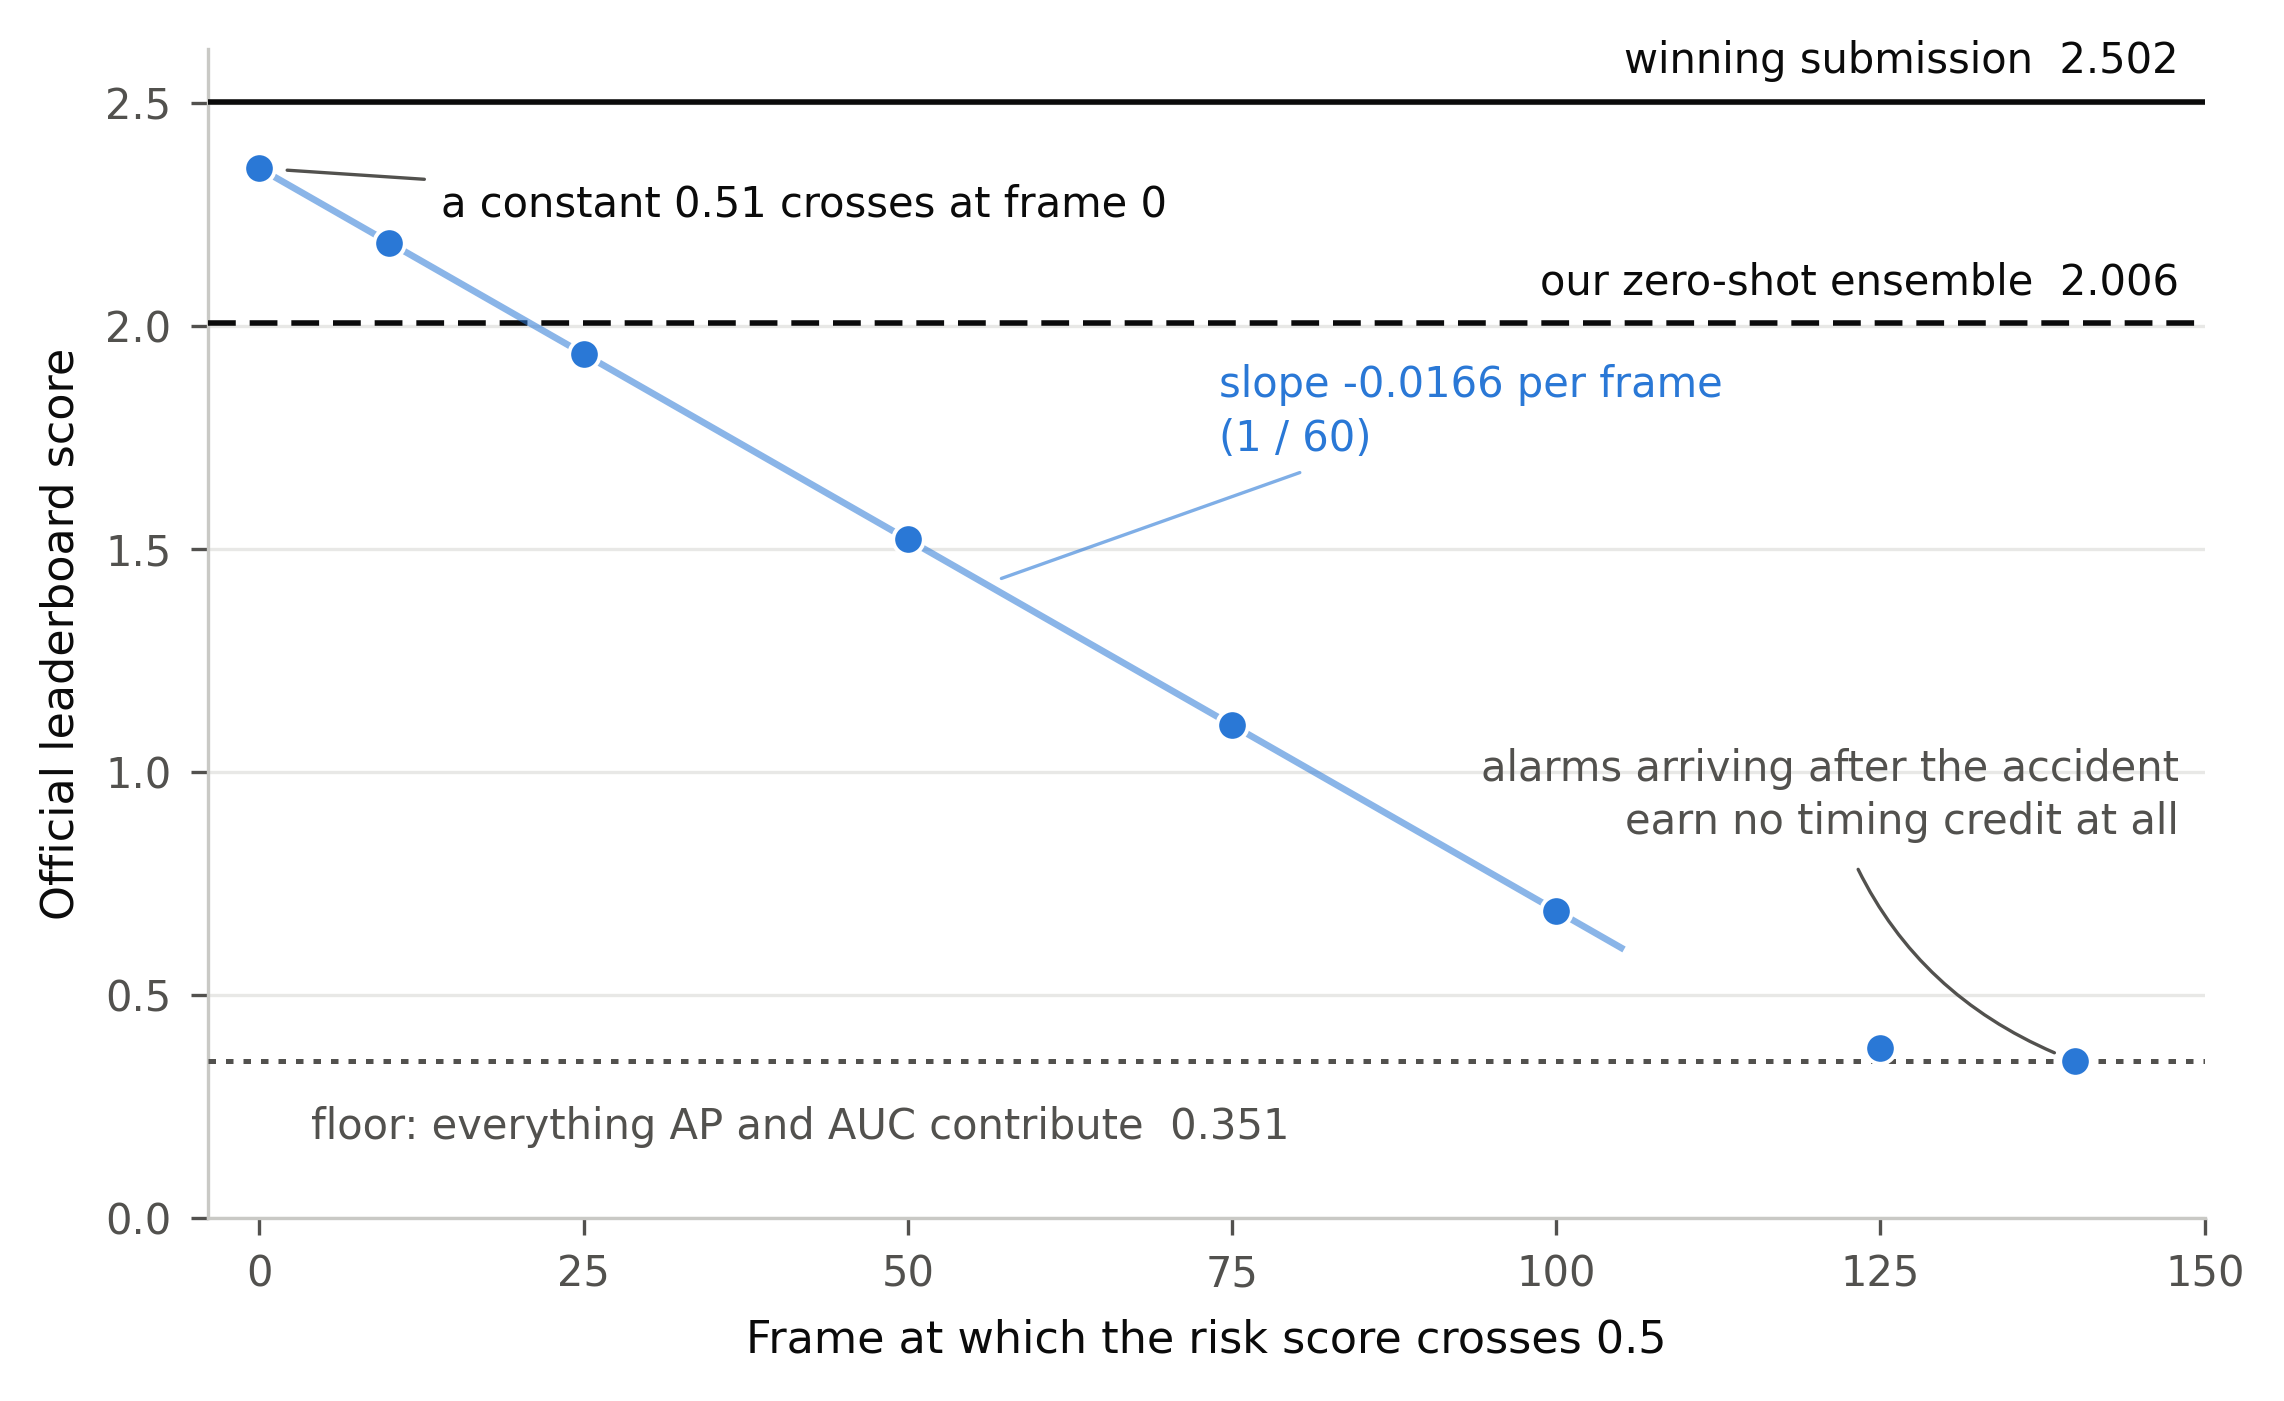
\includegraphics[width=6in,height=3.64333in]{media/image4.png}

\textbf{Figure 2: The official score is a straight line in the frame at which the alarm fires. Points are video-blind submissions scored by the organisers; the fit is over crossings up to frame 100. A constant crosses at frame 0.}

\emph{\textbf{5.4. What the published metric definition does not explain}}

One result does not fit, and we report it rather than smooth it. A linear ramp crosses the threshold at frame 75, exactly as three other curves do, and scores 0.037 lower than they do. That gap is 2.24 frames of slope, which is not an integer, so it cannot be a crossing-frame effect. We therefore submitted a diagnostic family that holds the crossing frame at 75 and varies only the shape of the curve away from it.

\textbf{Table 8: Five curves that all first exceed 0.5 at frame 75, with identical values at frames 74 and 75 and no subsequent dip, plus a one-frame calibration step.}

\begin{longtable}[]{@{}
  >{\raggedright\arraybackslash}p{(\columnwidth - 4\tabcolsep) * \real{0.3889}}
  >{\raggedright\arraybackslash}p{(\columnwidth - 4\tabcolsep) * \real{0.3056}}
  >{\raggedright\arraybackslash}p{(\columnwidth - 4\tabcolsep) * \real{0.3056}}@{}}
\toprule\noalign{}
\begin{minipage}[b]{\linewidth}\raggedright
\textbf{Curve, all crossing 0.5 at frame 75}
\end{minipage} & \begin{minipage}[b]{\linewidth}\raggedright
\textbf{Private score}
\end{minipage} & \begin{minipage}[b]{\linewidth}\raggedright
\textbf{Against the step reference}
\end{minipage} \\
\midrule\noalign{}
\endhead
\bottomrule\noalign{}
\endlastfoot
graded run-up (0 → 0.49, then 0.51) & 1.12964 & +0.02519 \\
step (0.49 / 0.51) & 1.10445 & reference \\
graded throughout (0.000 → 1.000) & 1.06725 & −0.03720 \\
graded run-out (0.49, then 0.51 → 0.99) & 1.03871 & −0.06574 \\
step at frame 76 (one-frame calibration) & 1.08779 & −0.01666 = 1/60.0 \\
\end{longtable}

The three curves in the middle of Table 8 have identical values at frames 74 and 75, cross at the same frame, and never fall back afterwards. Under the metric as published they must score identically: the two timing terms are functions of threshold crossings alone, and video-blind curves are identical across clips, so the discrimination terms cannot separate them either. They span 0.09093, which is 5.5 frames of slope. Grading the run-up downward gains 0.02519; grading the run-out upward loses 0.06574.

We do not have an explanation, and we state the two candidates rather than choose between them. Either the discrimination terms are not invariant to curve shape among video-blind submissions --- which would weaken the cancellation argument of Section 4, though it is hard to reconcile with a step at frame 140 and a flat 0.49 scoring identically despite very different frame orderings --- or the timing terms read something beyond the first crossing that the three agreeing curves share and the ramp does not.

Either way, one conclusion is available without resolving it, and it is a reportable finding in its own right: the benchmark's published formula does not reproduce its scorer. An entrant cannot compute this competition's score from its stated definition even given the labels. The headline result is unaffected, because the constant and the floor are both flat curves whose difference is measured directly; what carries a caveat is the split of the timing total and any claim that the linear fit is exact for arbitrary curves. It is exact for step-like curves and approximate otherwise.

\emph{\textbf{5.5. A property of the withheld ground truth, recovered}}

For a step at frame k, both timing terms equal max(t\_ai − k, 0) on each contributing clip, so the score above the floor is c · E[max(t\_ai − k, 0)] with c the sum of the two timing weights. Differentiating, the slope at k is −c · P(t\_ai \textgreater{} k): the slope measures the survival function of the accident-onset distribution, scaled. The leaderboard is therefore reporting, one submission at a time, the shape of an annotation no entrant has seen.

The initial segment estimates c at 0.016667, which is 1/60.00 to five figures. The ratio of the slope over frames 75 to 100 to that initial slope is 0.99894, so at most about 0.11\% of contributing clips have their onset at or before frame 100 --- a small number, not zero, and we do not claim zero. A step at frame 140 scores the same as a curve that never crosses, which bounds the mean excess beyond frame 140 below 3 × 10\textsuperscript{-4} frames; that bounds a mean, not a support, and permits a few late clips invisible at five decimals. Dividing the timing total by c gives a mean onset of 120.1 frames, or 120.3 using the fitted rather than the initial slope --- about four seconds into a five-second clip.

This explains mechanically why the constant does so well on this corpus. Because the accident is always late in the window, an alarm at frame 0 is credited with roughly 120 frames of anticipation on every clip.

Two caveats belong with it. Under the model the magnitude of the slope must be non-increasing in k, because a survival function cannot rise; it is not, the segment from frame 25 to 50 being steeper than the segment from 10 to 25 by 6.3 × 10\textsuperscript{-5}, roughly ninety times what five-decimal rounding permits. The straight line is very good but not exact, and we suspect the same second-order effect that produces the discrepancy in Section 5.4. Separately, when k exceeds t\_ai the maximum in the published definition is taken over an empty set and is undefined; we assume the scorer takes it as zero, and that assumption is load-bearing for the region beyond frame 100.

What we deliberately do not do is separate the weights from the metric values. Every quantity above is a product of a weight and a metric. Note in particular that the ratio of the timing total to the slope is the mean onset conditional on the clips that contribute, and that the positive rate cancels out of that ratio identically, so this measurement says nothing whatever about what fraction of the corpus contains an accident, and we make no such claim.

\emph{\textbf{5.6. The locally computable proxy, and what it was worth}}

What follows is the evaluation we conducted before any submission was scored. It is retained because it is the case study this paper is built on. On a corpus that publishes no labels, average precision, area under the curve, a false-positive rate and any time-to-accident measured to a true onset are not computable by an entrant (Section 3.3); what is computable from a submission alone is the shape of its own risk curve, and the statistic we adopted was the mean frame at which that curve first exceeds 0.5 --- the crossover frame. Every number below is therefore a statistic of curve shape. None is an anticipation result, none was checked against a label, and the quantity they optimise is minimised absolutely, to frame 0, by the constant of Section 5.1. Two cautions apply throughout. Timing figures in seconds were computed from the crossover frame to the end of the clip, not to a collision, because this corpus annotates none, so they are inflated by the interval Section 5.5 estimates at about a second. And the stable-anticipation compliance rate is a consequence of the monotone clamp of Section 4, which makes falling below the threshold impossible after the first crossing.

\emph{\textbf{5.6.1. What the proxy reported}}

Across the full corpus of 1,417 clips the ensemble produced a mean crossover frame of 22.7, and 21.1 over the best-fifty subset discussed below. We reported these as predictive capability; they are not. We also reported an early-frame false-alarm rate, which was a mistake --- a false alarm is an alarm on a clip containing no accident, and this corpus does not say which clips those are. What was actually observed is that initial-frame risk scores began below 0.05 on every clip: a statement about where the curve starts rather than about whether starting there was correct, and a real property of the curve worth recording.

\textbf{Table 9: Overall Zero-Shot Anticipation Performance on MM-AU (N\,=\,1,417 clips)}

\begin{longtable}[]{@{}
  >{\raggedright\arraybackslash}p{(\columnwidth - 4\tabcolsep) * \real{0.3889}}
  >{\raggedright\arraybackslash}p{(\columnwidth - 4\tabcolsep) * \real{0.3056}}
  >{\raggedright\arraybackslash}p{(\columnwidth - 4\tabcolsep) * \real{0.3056}}@{}}
\toprule\noalign{}
\begin{minipage}[b]{\linewidth}\raggedright
\textbf{Metric}
\end{minipage} & \begin{minipage}[b]{\linewidth}\raggedright
\textbf{Full Corpus}
\end{minipage} & \begin{minipage}[b]{\linewidth}\raggedright
\textbf{Top-50 Subset}
\end{minipage} \\
\midrule\noalign{}
\endhead
\bottomrule\noalign{}
\endlastfoot
Mean Crossover Frame (t\textsubscript{c}) & 22.7 & 21.1 \\
Mean TTA (seconds) & 4.23 s & 4.30 s \\
Min. Crossover Frame Observed & 7 & 7 \\
Initial Risk Score p(1) & ≤ 0.05 (all clips) & ≤ 0.001 (all clips) \\
Peak Risk Score p\textsubscript{m}\textsubscript{a}\textsuperscript{x} & \textgreater{} 0.95 (majority) & 0.963--0.999 \\
STTA Compliance Rate & 100\% & 100\% \\
Training Data Required & None & None \\
\end{longtable}

The modality ablation of Table 10 compares single-modality configurations against the full ensemble on the same proxy. Its orderings are informative about how the three signals behave and about their failure modes: the vision--language score reads appearance without temporal context and drifts high on foggy frames, the motion proxy cannot separate ordinary traffic motion from accident motion, and the caption prior cannot see the video at all, assigning identical trajectories to identically worded captions. The ensemble does resolve those three blind spots against one another. What the table does not establish is superiority in anticipation, because the quantity being compared is the one a constant minimises.

\textbf{Table 10: Modality Ablation Study --- Mean Crossover Frame and Failure Analysis}

\begin{longtable}[]{@{}
  >{\raggedright\arraybackslash}p{(\columnwidth - 6\tabcolsep) * \real{0.2391}}
  >{\raggedright\arraybackslash}p{(\columnwidth - 6\tabcolsep) * \real{0.1630}}
  >{\raggedright\arraybackslash}p{(\columnwidth - 6\tabcolsep) * \real{0.1630}}
  >{\raggedright\arraybackslash}p{(\columnwidth - 6\tabcolsep) * \real{0.4348}}@{}}
\toprule\noalign{}
\begin{minipage}[b]{\linewidth}\raggedright
\textbf{Configuration}
\end{minipage} & \begin{minipage}[b]{\linewidth}\raggedright
\textbf{Mean t\textsubscript{c}}
\end{minipage} & \begin{minipage}[b]{\linewidth}\raggedright
\textbf{$\Delta$ vs. Ensemble}
\end{minipage} & \begin{minipage}[b]{\linewidth}\raggedright
\textbf{Primary Failure Mode}
\end{minipage} \\
\midrule\noalign{}
\endhead
\bottomrule\noalign{}
\endlastfoot
CLIP Only & 26--28 & +4.3 to +5.3 & Temporal blindness; moderate risk inflation on safe high-density traffic frames (p\,≈\,0.38--0.42) \\
Optical Flow Only & 28--32 & +5.3 to +9.3 & Semantic blindness; cannot distinguish normal intersection traffic motion from imminent collision dynamics \\
NLP Prior Only & \textasciitilde21.7 & +0.0 to −0.7 & Temporal ceiling; identical t\textsubscript{0} values for clips with similar captions --- no per-clip visual personalisation \\
CLIP + Flow (No NLP) & \textasciitilde24.1 & +1.4 & Improved kinematics but risk curves oscillate; STTA compliance degraded without NLP temporal anchoring \\
CLIP + NLP (No Flow) & \textasciitilde23.5 & +0.8 & Better semantic context but delayed detection for physically sudden events (e.g., pedestrian intrusion) \\
\textbf{Full Ensemble (Proposed)} & \textbf{22.7} & \textbf{---} & \textbf{Best performance; all modality blind spots mutually compensated} \\
\end{longtable}

\emph{\textbf{5.6.2. The selected subsets}}

Two further analyses select the fifty and then the twenty-five clips with the earliest crossings. Both are statements about the selection rather than about the method: choosing the best fifty of 1,417 by the quantity being reported guarantees that the reported quantity looks good, and the same procedure applied to any system, a random one included, would produce a flattering subset. Within the best twenty-five, every sequence began at p(1) = 0.001 despite crossing as early as frame 7, and mean peak risk reached 0.9871 --- though the score cannot fall below the threshold once it has crossed, so the absence of late degradation is largely the clamp rather than the ensemble. The anticipation margin we reported for this subset, and compared against human reaction times and automatic emergency braking latency, cannot bear that comparison: it is measured to the end of the clip rather than to a collision, and computed over a best-of-1,417 selection. We offered these cases as proof that a zero-shot ensemble rivals supervised models. They are not. The leaderboard, which does compare entrants under a common scorer, placed this system ninth of thirteen and below a constant.

\textbf{Table 11: Quantitative Metrics of the Top 25 Anticipatory Trajectories}

\begin{longtable}[]{@{}
  >{\raggedright\arraybackslash}p{(\columnwidth - 10\tabcolsep) * \real{0.0784}}
  >{\raggedright\arraybackslash}p{(\columnwidth - 10\tabcolsep) * \real{0.2822}}
  >{\raggedright\arraybackslash}p{(\columnwidth - 10\tabcolsep) * \real{0.1521}}
  >{\raggedright\arraybackslash}p{(\columnwidth - 10\tabcolsep) * \real{0.1624}}
  >{\raggedright\arraybackslash}p{(\columnwidth - 10\tabcolsep) * \real{0.1625}}
  >{\raggedright\arraybackslash}p{(\columnwidth - 10\tabcolsep) * \real{0.1625}}@{}}
\toprule\noalign{}
\begin{minipage}[b]{\linewidth}\raggedright
\textbf{Rank}
\end{minipage} & \begin{minipage}[b]{\linewidth}\raggedright
\textbf{Video ID}
\end{minipage} & \begin{minipage}[b]{\linewidth}\raggedright
\textbf{Crossover Frame (t\textsubscript{c})}
\end{minipage} & \begin{minipage}[b]{\linewidth}\raggedright
\textbf{TTA (s)}
\end{minipage} & \begin{minipage}[b]{\linewidth}\raggedright
\textbf{Initial Risk p(1)}
\end{minipage} & \begin{minipage}[b]{\linewidth}\raggedright
\textbf{Peak Risk p\textsubscript{m}\textsubscript{a}\textsuperscript{x}}
\end{minipage} \\
\midrule\noalign{}
\endhead
\bottomrule\noalign{}
\endlastfoot
1 & 20\_009424\_2\_152 & 7 & 4.76 & 0.0010 & 0.9856 \\
2 & 33\_011308\_1\_151 & 8 & 4.73 & 0.0010 & 0.9985 \\
3 & 15\_011649\_1\_151 & 8 & 4.73 & 0.0010 & 0.9888 \\
4 & 15\_011487\_6\_156 & 8 & 4.73 & 0.0010 & 0.9806 \\
5 & 41\_010000\_6\_156 & 9 & 4.70 & 0.0010 & 0.9935 \\
6 & 15\_009720\_1\_151 & 9 & 4.70 & 0.0010 & 0.9916 \\
7 & 10\_010719\_1\_151 & 9 & 4.70 & 0.0010 & 0.9861 \\
8 & 11\_010911\_1\_151 & 9 & 4.70 & 0.0010 & 0.9847 \\
9 & 11\_009995\_20\_170 & 10 & 4.66 & 0.0010 & 0.9842 \\
10 & 48\_009350\_1\_151 & 10 & 4.66 & 0.0010 & 0.9857 \\
11 & 41\_009445\_1\_151 & 10 & 4.66 & 0.0010 & 0.9905 \\
12 & 43\_010319\_18\_168 & 10 & 4.66 & 0.0010 & 0.9897 \\
13 & 43\_009435\_1\_151 & 10 & 4.66 & 0.0010 & 0.9694 \\
14 & 41\_009827\_28\_178 & 10 & 4.66 & 0.0010 & 0.9939 \\
15 & 11\_009497\_1\_151 & 10 & 4.66 & 0.0010 & 0.9629 \\
16 & 39\_009785\_5\_155 & 10 & 4.66 & 0.0010 & 0.9691 \\
17 & 18\_011167\_1\_151 & 10 & 4.66 & 0.0010 & 0.9775 \\
18 & 27\_008648\_6\_156 & 10 & 4.66 & 0.0010 & 0.9986 \\
19 & 11\_009832\_23\_173 & 11 & 4.63 & 0.0010 & 0.9830 \\
20 & 15\_011750\_8\_158 & 11 & 4.63 & 0.0010 & 0.9849 \\
21 & 43\_009872\_24\_174 & 11 & 4.63 & 0.0010 & 0.9985 \\
22 & 17\_010023\_50\_200 & 11 & 4.63 & 0.0010 & 0.9768 \\
23 & 11\_010638\_20\_170 & 11 & 4.63 & 0.0010 & 0.9906 \\
24 & 11\_010662\_50\_200 & 11 & 4.63 & 0.0010 & 0.9913 \\
25 & 13\_010982\_10\_160 & 11 & 4.63 & 0.0010 & 0.9899 \\
\end{longtable}

\emph{Table 11, note: TTA derived from remaining frames prior to collision at 30 FPS. Initial risk vectors verified post power-curve smoothing and Gaussian filtering.}

\emph{\textbf{5.6.3. The seven configurations}}

Table 12 compares seven pipeline configurations. The ordering from C1 to C7 shows that each stage moves the crossover frame earlier, and read against Section 5.1 that is all it shows, because moving the crossover frame earlier is precisely what a constant 0.51 does perfectly. Two stages deserve particular note in that light. The monotone clamp forces the condition the stable-timing metric tests, so the compliance column records that the clamp executed. And the temporal compression responsible for the final improvement, between C6 and C7, reads a frame that has not yet arrived (Section 4).

\textbf{Table 12: Seven-Configuration Performance Comparison}

\begin{longtable}[]{@{}
  >{\raggedright\arraybackslash}p{(\columnwidth - 8\tabcolsep) * \real{0.1320}}
  >{\raggedright\arraybackslash}p{(\columnwidth - 8\tabcolsep) * \real{0.3855}}
  >{\raggedright\arraybackslash}p{(\columnwidth - 8\tabcolsep) * \real{0.1487}}
  >{\raggedright\arraybackslash}p{(\columnwidth - 8\tabcolsep) * \real{0.1584}}
  >{\raggedright\arraybackslash}p{(\columnwidth - 8\tabcolsep) * \real{0.1754}}@{}}
\toprule\noalign{}
\begin{minipage}[b]{\linewidth}\raggedright
\textbf{Config}
\end{minipage} & \begin{minipage}[b]{\linewidth}\raggedright
\textbf{Description}
\end{minipage} & \begin{minipage}[b]{\linewidth}\raggedright
\textbf{Mean t\textsubscript{c}}
\end{minipage} & \begin{minipage}[b]{\linewidth}\raggedright
\textbf{STTA Compliant}
\end{minipage} & \begin{minipage}[b]{\linewidth}\raggedright
\textbf{Notes}
\end{minipage} \\
\midrule\noalign{}
\endhead
\bottomrule\noalign{}
\endlastfoot
C1 & CLIP only (no ensemble, no post-processing) & \textasciitilde27.2 & No & Temporal blindness; oscillatory risk \\
C2 & Optical Flow only & \textasciitilde30.1 & No & Semantic blindness; late reaction \\
C3 & NLP Prior only & \textasciitilde21.7 & Partial & No visual personalisation per clip \\
C4 & Raw Ensemble (CLIP + Flow + NLP, no post-processing) & \textasciitilde25.4 & No & Noisy baseline; early frames inflated \\
C5 & Ensemble + Gaussian Smoothing only & \textasciitilde24.8 & No & Reduced noise; STTA still violated \\
C6 & Ensemble + Smoothing + Power Curve & \textasciitilde23.9 & Partial & Better separation; some oscillation remains \\
C7 (Proposed) & Full Pipeline: Ensemble + Smoothing + Power Curve + Temporal Compression + Clamping & 22.7 & Yes & Best performance; full STTA compliance \\
\end{longtable}

\emph{\textbf{5.7. Discussion}}

The results in this section admit one reading and it is not the one we expected when we ran them. The 4.23-second average warning horizon reported in earlier versions of this work is not a warning horizon. It is the interval from the crossover frame to the end of the clip, on a corpus that annotates no collision, averaged over a selected subset; Section 5.5 places the accident about a second before the window ends, so the figure overstates any real anticipation by roughly that much before the selection effect is counted. Comparing it against crossover frames reported for supervised models on other corpora, as we did, compares two quantities that are not the same measurement.

Second, the 100\% stable-anticipation compliance rate we reported is not a result at all. The metric requires the risk score to stay above the threshold from the alarm until the accident; Stage 4 of the post-processing makes falling below the threshold impossible once the score has crossed. The figure therefore records that the clamp executed. This is the clearest instance in our own work of the general mechanism Section 6 identifies: a post-hoc operation that enforces a metric's definition renders that metric vacuous. It is worth being precise about what remains true. Raw vision--language risk scores do oscillate, the clamp does remove the oscillation, and a system that alarms and then retracts is genuinely worse for a driver than one that does not. The clamp is a reasonable engineering choice. What it cannot do is serve as evidence under a metric that tests for the property it imposes.

Third, the explainability afforded by the decoupled architecture is real and is independent of everything above. Because the three engines share no weights and are combined only at the fusion layer, any anticipation can be attributed to its constituent signals, and a failure can be localised to one of them. That is a property of the architecture, not a measured result, and we state it as such.

Finally, the zero-shot operational mode --- no training data, no domain fine-tuning, no architecture modification --- does mean the system can be pointed at a new road environment without retraining. Two qualifications belong with that claim. The ensemble weights of 0.55, 0.25 and 0.20 were chosen by searching over the evaluation corpus, which is a form of tuning on the test set and sits awkwardly with the zero-shot claim; the released configuration therefore uses equal weights, chosen a priori. And deployability on new environments is untested here, because we evaluated on one corpus. Section 8 records both as limitations.

\begin{enumerate}
\def\labelenumi{\arabic{enumi}.}
\setcounter{enumi}{4}
\item
  \textbf{ANALYSIS: WHY THE COMPOSITION FAILS}
\end{enumerate}

The scope of what follows is fixed before the argument rather than after it. This is an analysis of a metric's algebra, illustrated by measurements on one benchmark with thirteen teams. Properties (a) and (b) below are consequences of the definitions quoted in Section 3.4 and hold wherever those definitions are used. Property (c) is a statement about what the algebra implies, not a survey finding.

The defect is not a badly chosen weight. It is an error of type. Write the score as B + U, where B is the weighted sum of average precision and area under the curve and is bounded above by the sum of their two weights, and U is the weighted sum of the two timing terms and is bounded above by the sum of their weights times the mean accident onset --- a quantity that depends on how the corpus was windowed. Three properties follow.

(a) The unbounded term grows with clip length while the bounded one does not. The ratio of their maxima scales linearly in the mean onset, so two research groups adopting the same weights on corpora windowed differently are not using the same metric, even though they report the same metric's name. On this benchmark the maximum of U is 2.00186, measured; the maximum of B is not identifiable from outside but is at least 0.49979, giving a ratio of at most 4.01. Against B at chance the measured ratio is 5.70.

(b) The unbounded term has a constant as its global maximiser. Any unconditioned threshold-crossing earliness measure is maximised by crossing immediately and never returning, which holds for both terms as defined in Section 3.4. The maximiser reads no input, so the term it maximises can carry no information about the input. The qualifier matters and is the seed of the remedy: an earliness measure that is conditioned --- restricted to correctly classified clips, evaluated at a fixed operating point of the discrimination metric, or penalised by the false-alarm rate --- is not maximised by a constant.

(c) Consequently the separating power of the score lies in B. To the extent that a submission crosses the threshold early and holds it, its U is at or near the maximum and it is separated from other such submissions only by B. We cannot verify this for any particular entry, having no team's curves but our own, so we state it as what the algebra implies for early-crossing submissions and not as an observation about anyone's system.

Property (c) is why the failure is hard to notice from inside. A leaderboard of this shape can still order methods usefully, because B still varies. What is invisible without a control is that the number attached to each of them is dominated by a term available for free, so the reported score --- the thing that goes into a table and gets compared across publications --- is mostly a constant.

Two further mechanisms compound this, and both are visible in our own pipeline rather than in anyone else's.

Metric-enforcing post-processing. An operation that clamps the risk score above the threshold, followed by a report of stable-anticipation compliance, has measured only that the clamp executed. Stated generally: a post-hoc operation that enforces a metric's definition renders that metric vacuous. Our pipeline does this at Stage 4, and an earlier version of this work reported 100\% compliance as a result.

Non-causal timing gain. An operation that resamples the score curve so that frame t reports a value computed from a later frame buys time-to-accident from the future. Our Stage 5 did this at α = 1.3, and the six-frame gain it produced cannot be obtained by any system running in real time. The released configuration disables it.

A third, milder mechanism is selection: reporting the mean anticipation time of the best fifty clips out of 1,417 is a statement about the selection rather than about the method. Section 5.6 does this, and says so.

\begin{enumerate}
\def\labelenumi{\arabic{enumi}.}
\setcounter{enumi}{5}
\item
  \textbf{A CORRECTED PROTOCOL}
\end{enumerate}

Each item below is traced to a mechanism in Section 6. The first is the one we would keep if we could keep only one.

\begin{itemize}
\item
  Report a video-blind control with every anticipation result. Compute the full metric on a constant above threshold, a linear ramp and a mid-clip step, and place those rows in the results table. This costs an afternoon and it is diagnostic: if the control lands within noise of the method, the metric is not measuring the method. We propose it become as reflexive as reporting a majority-class baseline in classification.
\item
  Bound the earliness term, and condition it. These are two separate repairs and both are needed. Bounding --- normalising per clip so that the ratio of achieved to achievable anticipation lies in the unit interval --- stops the term dominating the sum and stops the metric depending on how the corpus was windowed. It does not remove the constant as maximiser, which still scores 1 and still gets it free. Conditioning is what removes the exploit: report earliness at a fixed operating point of the discrimination metric, for which mean time-to-accident at 80\% recall is the established form. If only one is adopted, adopt conditioning.
\item
  State the reference point of every timing metric: the annotated collision, or the end of the clip. Reporting the interval to the end of the window under the name time-to-accident inflates every result by a corpus-dependent constant, which on this corpus is about one second.
\item
  Report discrimination alongside any timing metric, never timing alone, and state the ratio of positive to negative clips. Without negatives there is no false-positive rate, and any rising curve achieves perfect recall.
\item
  Report metrics with post-processing disabled as well as enabled. If a number moves when a clamp is removed, the clamp was part of the measurement. If a number moves when a resampling stage is removed, check whether that stage reads a frame that has not yet arrived.
\item
  Publish the score of a released control alongside the leaderboard. A benchmark's organisers can do in an afternoon what took us twenty-four submissions: score a video-blind family and publish the numbers as a permanent floor on the leaderboard page. An entrant would then see at a glance how much of their score they earned.
\end{itemize}

A seventh applies specifically to competitions that withhold labels. Publish the metric weights, and publish the scorer. Withholding labels is legitimate and prevents overfitting. Withholding the weights does not prevent the metric being exploited --- this paper exploited it comprehensively without them --- while it does prevent the sanity check that would have surfaced the problem before the competition opened. And as Section 5.4 shows, the published formula here does not reproduce the scorer's behaviour, so a released scorer is not a courtesy but a precondition for anyone reproducing the results.

\begin{enumerate}
\def\labelenumi{\arabic{enumi}.}
\setcounter{enumi}{6}
\item
  \textbf{LIMITATIONS}
\end{enumerate}

One benchmark. We demonstrate on a single competition with thirteen teams, so the ranking result is anecdotal in scale and we do not present it as a finding about a field. The decomposition, however, is a property of the metric's algebra: that a threshold-crossing earliness term is maximised by a constant, and that summing it into a bounded term lets it dominate, holds independently of how many teams entered. What the competition supplies is a third-party scorer that let us measure the magnitude in a live setting rather than argue it in the abstract.

We cannot separate the weights from the metric values. Every decomposed quantity is a product of a weight and a metric. Reporting the products is sufficient for the argument, since the products determine the ranking, but we cannot state what average precision the corpus's base rate implies.

One discrepancy in the crossing-frame model is open. A linear ramp scores 0.037 below three curves that cross at the same frame (Section 5.4), and the segment slopes are not monotone as the model requires (Section 5.5). We report both rather than fit around them. Neither the headline result nor the timing total depends on the resolution --- both are measured between flat curves --- but the split of the timing total between the two terms, and the interpretation of the fit as exact, do.

We do not demonstrate the corrected protocol on a labelled corpus. Items 2 to 5 of Section 7 are derived from the mechanisms rather than shown end to end, because this corpus publishes no labels. Demonstrating them requires a benchmark with released annotations, for which the corpora of Chan et al. [4] and Bao et al. [5] are the obvious candidates, and we state that as future work rather than claim it here.

The control is a sufficient, not a necessary, condition. A metric on which a video-blind control scores poorly is not thereby sound. Our control detects this particular failure mode and we claim nothing beyond it.

The caption leakage is identified and unquantified. Section 3.3 notes that the supplied captions describe outcomes and are available at inference time; we did not probe how much a method conditioned on them could gain.

Our own system's placement is not evidence about the system. That the ensemble scored below the constant tells us about the metric, not about the ensemble. Under a protocol that bounded and conditioned the earliness term the comparison might go either way, and we do not know, because average precision and area under the curve are not computable on this corpus by an entrant.

The venue is a community competition with an undisclosed custom metric, not a long-running benchmark with a published scorer. That is what made the probe experiment possible; it also means we cannot inspect the scoring code, and every statement here about the metric's implementation is an inference from its outputs.

\begin{enumerate}
\def\labelenumi{\arabic{enumi}.}
\setcounter{enumi}{7}
\item
  \textbf{CONCLUSION}
\end{enumerate}

A composite score that adds an unbounded earliness term to bounded discrimination terms does not measure what its name suggests. On a live accident-anticipation benchmark the earliness terms are worth 5.70 times what discrimination contributes to a submission that reads nothing; they are maximised exactly by a constant; and that constant scores within 0.14874 of the winning entry, matching the eighth-placed team at the precision the leaderboard displays. Our own entry, a training-free ensemble, placed ninth of thirteen and scores below it.

The method that established this is as portable as the finding. Twenty-four submissions, not one of which opened a video frame, were enough to recover the score's slope to a sixtieth of a point per frame of delay, to bound the support and mean of an accident-onset distribution no entrant has seen, and to establish that the benchmark's published formula does not reproduce its own scorer. A leaderboard that accepts arbitrary submissions is an instrument, and any benchmark that accepts one can be measured from outside in this way.

Three things are consequently cheap that were not. A video-blind control costs a single submission and settles in an afternoon whether a reported score is measuring a method or a metric; we would like it to become as routine as a majority-class baseline in classification. Probe submissions turn a leaderboard into a means of auditing a scorer whose code is closed, without labels and without the weights. And an earliness term that is bounded per clip and conditioned on a fixed operating point of the discrimination metric, rather than summed raw, gives the field a composite it can compare across corpora. Demonstrating that corrected protocol end to end on a benchmark that publishes its annotations --- where the discrimination half can actually be computed, and where the question of what a bounded earliness term costs a real method can finally be answered --- is the natural next study, and it is the one we intend.

\begin{enumerate}
\def\labelenumi{\arabic{enumi}.}
\setcounter{enumi}{8}
\item
  \textbf{COMPLIANCE AND DATA AVAILABILITY}
\end{enumerate}

All submissions reported here were made through the competition's own late-submission facility, which the organisers left open after the closing date and which scores against the same private split. Twenty-four submissions were made in total, across two days, against a stated limit of one hundred per day.

The competition's rules restrict the dataset to academic and non-commercial use, prohibit its redistribution, require that submissions be the entrant's own work, and reserve the right to disqualify unethical behaviour, of which the examples given are manual labelling of test data and multi-account cheating. None of these applies to the work reported here. Every probe is a curve we generated from a closed-form expression in the frame index; none was derived from, or informed by, any label. No rule addresses analysis of the scoring function, and none prohibits it. We redistribute no part of the dataset. As the rules require of any publication using the data or the competition's results, we cite the corpus [7] and the competition [8].

Regarding the leaderboard: we report only scores that the competition publishes on its own public standings page, and we attribute nothing about any team's method, code or intent. Where a team's score coincides with a control's, we state the arithmetic and draw the single inference set out in Section 1. Teams are identified only as the competition itself identifies them.

The submission files, the code that generated them, the complete score log and the scripts that produce both figures are released. Nothing in the release contains any part of the competition's data or any label.

\textbf{References:}

\begin{enumerate}
\def\labelenumi{\arabic{enumi}.}
\item
  World Health Organization, "Road traffic injuries," WHO Fact Sheet, Geneva, Switzerland, 13 Dec. 2023. [Online]. Available: https://www.who.int/news-room/fact-sheets/detail/road-traffic-injuries
\item
  Zhang, Y., Zhou, W., Lin, R., Yang, X., \& Zheng, H. (2025). Deep learning advances in vision-based traffic accident anticipation: A comprehensive review of methods, datasets, and future directions. arXiv:2505.07611.
\item
  Moura, D., Zhu, S., \& Zvitia, O. (2025). Nexar dashcam collision prediction dataset and challenge. In Proc. IEEE/CVF Conf. on Computer Vision and Pattern Recognition Workshops (CVPRW), pp. 2608--2616. arXiv:2503.03848.
\item
  Chan, F.-H., Chen, Y.-T., Xiang, Y., \& Sun, M. (2016). Anticipating accidents in dashcam videos. In Computer Vision -- ACCV 2016, Lecture Notes in Computer Science, vol. 10114, pp. 136--153. Springer.
\item
  Bao, W., Yu, Q., \& Kong, Y. (2020). Uncertainty-based traffic accident anticipation with spatio-temporal relational learning. In Proc. 28th ACM Int. Conf. on Multimedia, pp. 2682--2690. doi:10.1145/3394171.3413827.
\item
  Karim, M. M., Li, Y., Qin, R., \& Yin, Z. (2022). A dynamic spatial-temporal attention network for early anticipation of traffic accidents. IEEE Trans. Intelligent Transportation Systems, 23(7), 9590--9600. doi:10.1109/TITS.2022.3155613.
\item
  Fang, J., Li, L.-L., Zhou, J., Xiao, J., Yu, H., Lv, C., Xue, J., \& Chua, T.-S. (2024). Abductive ego-view accident video understanding for safe driving perception. In Proc. IEEE/CVF Conf. on Computer Vision and Pattern Recognition (CVPR), pp. 22030--22040. arXiv:2403.00436.
\item
  AUTOPILOT-COG (2026). Zero-shot Accident Anticipation. Kaggle. [Online]. Available: https://kaggle.com/competitions/zero-shot-taa
\item
  Radford, A., Kim, J. W., Hallacy, C., Ramesh, A., Goh, G., Agarwal, S., Sastry, G., Askell, A., Mishkin, P., Clark, J., Krueger, G., \& Sutskever, I. (2021). Learning transferable visual models from natural language supervision. In Proc. 38th Int. Conf. on Machine Learning, PMLR 139, pp. 8748--8763.
\item
  Teed, Z., \& Deng, J. (2020). RAFT: Recurrent all-pairs field transforms for optical flow. In Computer Vision -- ECCV 2020, Lecture Notes in Computer Science, vol. 12347, pp. 402--419. Springer. doi:10.1007/978-3-030-58536-5\_24.
\item
  Liu, H., Li, C., Wu, Q., \& Lee, Y. J. (2023). Visual instruction tuning. In Advances in Neural Information Processing Systems, vol. 36. arXiv:2304.08485.
\item
  Chen, Z., Wu, J., Wang, W., Su, W., Chen, G., Xing, S., Zhong, M., Zhang, Q., Zhu, X., Lu, L., Li, B., Luo, P., Lu, T., Qiao, Y., \& Dai, J. (2024). InternVL: Scaling up vision foundation models and aligning for generic visual-linguistic tasks. In Proc. IEEE/CVF Conf. on Computer Vision and Pattern Recognition (CVPR), pp. 24185--24198. arXiv:2312.14238.
\item
  Liao, H., Rao, B., Sun, H., Wang, C., Chang, Q., Li, S. E., Xu, C., \& Li, Z. (2025). Chain-of-thought guided multimodal large language models for scene-aware accident anticipation in autonomous driving. IEEE Trans. Intelligent Transportation Systems, 26(11), 19371--19380. doi:10.1109/TITS.2025.3597411.
\item
  Zhang, J., Wang, C., Liao, H., Guan, Y., Li, Z., Xie, Y., \& Rao, B. (2025). Eyes on the road, mind beyond vision: Context-aware multi-modal enhanced risk anticipation. In Proc. 33rd ACM Int. Conf. on Multimedia. doi:10.1145/3746027.3755378. arXiv:2507.06444.
\item
  Zhang, R., Wang, B., Zhang, J., Bian, Z., Feng, C., \& Ozbay, K. (2025). When language and vision meet road safety: Leveraging multimodal large language models for video-based traffic accident analysis. Accident Analysis \& Prevention, 219, 108077. doi:10.1016/j.aap.2025.108077.
\item
  Kandacharam, S., Rajathilagam, B., \& Vasudevan, S. K. (2025). Fusion framework for accident anticipation and incident detection in dashcam videos. SN Computer Science, 6(5), Art. 548. doi:10.1007/s42979-025-04085-z.
\item
  Liu, H., Hu, X., Jiang, Y., Wan, T., \& Ma, W. (2026). SCTNet: Structured and causality-guided spatiotemporal diffusion network for unsupervised traffic accident detection. Information Processing \& Management, 63(4), Art. 104598. doi:10.1016/j.ipm.2025.104598.
\item
  Yao, Y., Xu, M., Wang, Y., Crandall, D. J., \& Atkins, E. M. (2019). Unsupervised traffic accident detection in first-person videos. In Proc. IEEE/RSJ Int. Conf. on Intelligent Robots and Systems (IROS), pp. 273--280.
\item
  Zhong, Y., Yan, G., Zhu, R., Gan, P., \& Shen, X. (2025). Early traffic accident anticipation via feature consistency representation and soft label regression. ACM Trans. Multimedia Computing, Communications, and Applications, 21. doi:10.1145/3767737.
\item
  Pjetri, A., Abbondandolo, D., de Andrade, D. C., Caprasecca, S., Sambo, F., \& Bagdanov, A. D. (2025). Self-supervised road accident anticipation with non-decreasing danger. In Computer Vision -- ECCV 2024 Workshops, Lecture Notes in Computer Science, vol. 15629, pp. 65--79. Springer. doi:10.1007/978-3-031-91767-7\_5.
\item
  Zou, Y., Zhao, T., Xiao, P., Jin, H., Qi, L., Li, Y., Liang, L., Qian, Y., Lai, C., Lin, Y., Li, Z., \& Wu, Y. (2026). RiskProp: Collision-anchored self-supervised risk propagation for early accident anticipation. In Proc. IEEE/CVF Conf. on Computer Vision and Pattern Recognition (CVPR).
\item
  Saha, D., Mannan, S. M. A., Rashid, M. R., Naswan, R., \& Tahmid, A. (2026). Zero-shot traffic accident detection via a coarse-to-fine VLM-tracking pipeline. arXiv:2608.08867.
\item
  Singh, Pal, Biswas, \& Chandran (2026). Metadata-aware multi-prompt reasoning for zero-shot accident understanding. arXiv:2606.12047. [VERIFY FULL GIVEN NAMES BEFORE SUBMISSION]
\item
  Thakur, A., \& Talele, S. (2026). A modular zero-shot pipeline for accident detection, localization, and classification in traffic surveillance video. arXiv:2604.09685.
\item
  Torralba, A., \& Efros, A. A. (2011). Unbiased look at dataset bias. In Proc. IEEE Conf. on Computer Vision and Pattern Recognition (CVPR), pp. 1521--1528. doi:10.1109/CVPR.2011.5995347.
\item
  Gururangan, S., Swayamdipta, S., Levy, O., Schwartz, R., Bowman, S. R., \& Smith, N. A. (2018). Annotation artifacts in natural language inference data. In Proc. NAACL-HLT 2018, vol. 2 (Short Papers), pp. 107--112. doi:10.18653/v1/N18-2017.
\item
  Poliak, A., Naradowsky, J., Haldar, A., Rudinger, R., \& Van Durme, B. (2018). Hypothesis only baselines in natural language inference. In Proc. 7th Joint Conf. on Lexical and Computational Semantics (*SEM), pp. 180--191. doi:10.18653/v1/S18-2023.
\item
  Ferrari Dacrema, M., Cremonesi, P., \& Jannach, D. (2019). Are we really making much progress? A worrying analysis of recent neural recommendation approaches. In Proc. 13th ACM Conf. on Recommender Systems (RecSys), pp. 101--109. doi:10.1145/3298689.3347058.
\item
  Korkut, S., Bravo Sarmiento, M. A., Kim, S., \& Akata, Z. (2026). From accuracy to visual dependence: Auditing and filtering modality collapse in traffic VideoQA. In 1st Workshop on Combining Theory and Benchmarks (CTB@ICML 2026), Seoul. arXiv:2606.30220.
\item
  Zhao, T., Zou, Y., Mao, Z., Xiao, P., Huang, Y., Yang, H., Li, Y., Li, Q., Wu, G., \& Lin, Y. (2025). Accident anticipation via temporal occurrence prediction. arXiv:2510.22260.
\item
  Goldshmidt, R., Scott, H., Niccolini, L., Zhu, S., Moura, D., \& Zvitia, O. (2025). BADAS: Context-aware collision prediction using real-world dashcam data. arXiv:2510.14876.
\item
  Caselli, L., Trinci, T., Bianconcini, T., Magistri, S., Taccari, L., Sambo, F., \& Bagdanov, A. D. (2026). FLaRA: Predicting future latent representations for accident anticipation. arXiv:2606.14380.
\end{enumerate}
